% !TeX root = ../main.tex

\chapter{基于去噪扩散模型的水下图像增强算法}
水下图像由于红光快速衰减和悬浮颗粒的光散射作用,通常会出现显著的色偏和模糊。
这种质量退化严重限制了下游任务(如目标检测或语义分割)的表现,主要是由于可用的语义信息不足。
尽管基于生成对抗网络的图像增强方法在一定程度上缓解了这一问题,但其固有的对抗训练机制容易导致模式崩溃,限制了进一步提升效果的可能性。

为解决上述问题,本章提出一种基于水下图像补丁的去噪扩散模型水下图像增强算法。
该方法结合扩散模型的强大图像生成能力与补丁级别的采样策略,以提高处理效率和生成图像的细节质量。
算法基于扩散模型训练框架,以原始图像作为生成条件,设计了融合补丁引导采样的优化流程,并调整了扩散模型噪声估计网络结构以适配补丁级别的训练模式,从而提高去噪阶段的估计精度。
在实验部分详细介绍了所用数据及评价指标,并通过与多种现有方法的对比,系统验证了该方法在水下图像增强中的有效性。


% 水下图像往往由于红光的衰减与悬浮物的反射而出现严重的色偏与模糊,导致许多下游任务由于缺乏有效的语义信息而受到限制。
% 虽然基于生成对抗网络的方式已经取得了不错效果,但是会遭遇对抗训练固有的模式崩塌问题。
% 针对生成对抗网络的瓶颈,本章将介绍基于去噪扩散模型的水下图像增强算法。
% 利用基本的扩散模型训练框架,将原始图像作为生成条件,融合补丁引导的采样过程来提高模型的处理效率和图像细节,
% 并且重新设计了适用于补丁大小的U-Net网络结构来估计去噪阶段的噪声,
% 最后详细描述了实验数据和评价指标,通过与其他模型的对比,全面论证所提出的方法对水下图像增强的有效性。

\section{基于补丁引导的水下图像去噪扩散采样过程}
扩散模型因其学习图像先验的能力,在图像生成领域表现出色。
然而,现有扩散模型通常依赖于训练数据与测试数据分布的一致性。当两者分布不匹配时,生成的图像可能出现伪影或视觉假象。
为解决这一问题,本章提出一种基于水下图像补丁级别的去噪扩散方法。
通过将图像分解为小型补丁以学习局部的扩散先验,该方法显著降低了对整体图像分布的依赖,并通过实验验证其优于传统完整图像方法的表现。

\subsection{基于滑动窗口的补丁获取}
本文采用滑动窗口技术将图像分解为多个重叠补丁,以作为去噪扩散模型的输入。
滑动窗口的步长 $s$ 小于补丁大小 $p$,可以在补丁之间形成重叠,形成采样过程中的自然过渡,提高模型的图像重建质量。
然而,滑动窗口方法在特定步长和补丁大小的组合下,可能导致以下两种问题:
(1)边缘像素丢失:当窗口无法完全覆盖图像边缘部分时,会出现未裁剪区域。若简单用区域均值填充,可能扩散填充值误差,影响重建结果。
(2)尺寸不一致:直接丢弃边缘区域的像素会导致生成图像尺寸与原图不一致。
为解决上述问题,本文对图像边缘进行了额外分解,确保最终补丁集合能够完整覆盖整个图像,并避免图像完整像素的丢失。
\begin{algorithm}[ht]
\caption{补丁获取方法}
\label{alg:patch}
\KwIn{任意分辨率的图片输入 $\bm{X}$,滑动窗口的步长 $s$,补丁(窗口)大小 $p$,输入 $\bm{X}$ 的宽度 $W$ 和高度 $H$}
\KwOut{提取的补丁 $\mathbf{x}^{(i)}$}
\SetKwInOut{Input}{输入}
\SetKwInOut{Output}{输出}
\SetKw{KwTo}{to}
\SetKw{KwBy}{with step}

\SetKw{KwData}{数据}
\SetKw{KwResult}{结果}

$\bm{P} \gets \mathbf{0}$ \tcp{和图像 $\bm{X}$\; 大小一致的补丁掩码}
$i \gets 0$\; \tcp{补丁编号}

\For{$w = 0$ \KwTo $W - p$ \KwBy $s$}{
    \For{$h = 0$ \KwTo $H - p$ \KwBy $s$}{
        $\bm{P}_i \gets \bm{P}[0:end, h:h + p, w:w + p] + \mathbf{1}$\;
        $\mathbf{x}^{(i)} \gets \text{Crop}(\bm{P}_i \circ \bm{X})$\ $\mathbin{/\mkern-4mu//}$ $\circ$: 哈达玛积;
        $i \gets i + 1$\;
    }
}

$\mathbin{/\mkern-2mu/}$ 右侧边缘补丁获取\;
$w \gets W - p$\;

\For{$h = 0$ \KwTo $H - p$ \KwBy $s$}{
    $\bm{P}_i \gets \bm{P}[0:end, h:h + p, w:w + p] + \mathbf{1}$\;
    $\mathbf{x}^{(i)} \gets \text{Crop}(\bm{P}_i \circ \bm{X})$\;
    $i \gets i + 1$\;
}

$\mathbin{/\mkern-2mu/}$ 底部边缘补丁获取\;
$h \gets H - p$\;

\For{$w = 0$ \KwTo $W - p$ \KwBy $s$}{
    $\bm{P}_i \gets \bm{P}[0:end, h:h + p, w:w + p] + \mathbf{1}$\;
    $\mathbf{x}^{(i)} \gets \text{Crop}(\bm{P}_i \circ \bm{X})$\;
    $i \gets i + 1$\;
}

$\mathbin{/\mkern-2mu/}$ 右下部分补丁获取\;
$h \gets H - p$\;
$w \gets W - p$\;
$\bm{P}_i \gets \bm{P}[0:end, h:h + p, w:w + p] + \mathbf{1}$\;
$\mathbf{x}^{(i)} \gets \text{Crop}(\bm{P}_i \circ \bm{X})$\;
\end{algorithm}

如算法 \ref{alg:patch} 所示,补丁提取的过程由以下几个步骤组成:

首先,初始化一个与输入图像 $\bm{X}$ 尺寸一致的掩码 $\bm{P}$,用于标记补丁覆盖的区域。
在主循环中,通过滑动窗口的方式提取图像的主要补丁。
在每次迭代中,滑动窗口定位到当前区域,将对应的掩码 $\bm{P}$ 的覆盖区域值加 1,以记录该部分被提取的次数。
随后,利用哈达玛积(Hadamard Product)运算,裁剪出该位置的图像补丁。

在完成主要区域的补丁提取后,需要针对图像的边缘部分进一步分解。
为了处理右侧边缘、底部边缘以及右下角区域的剩余像素,单独执行补丁提取操作,
以确保每个像素都包含在提取的补丁中,避免出现信息丢失或分辨率不一致的问题。

最终,所有提取的补丁被存储在一个列表中,形成覆盖整个图像的补丁集合 ${\mathbf{x}^{(i)}}$。
这些补丁将作为去噪扩散模型的生成先验,在训练和推理时作为噪声估计网络的原始数据。

% 如算法\ref{alg:patch}所示,首先初始化一个与输入图像 $\bm{X}$ 相同大小的掩码 $\bm{P}$,然后通过滑动窗口的方式获取图像的主要补丁。
% 在每次迭代中,将掩码 $\bm{P}$ 的相应区域加1,然后通过哈达玛积运算获取对应位置的补丁。
% 在获取完整的补丁后,我们将其存储在一个列表中,以便后续的处理。
% 最后,再通过对图像边缘的额外分解,获取右侧边缘、底部边缘和右下部分的补丁。
% 这样可以获得覆盖整个图像的补丁集合,这些补丁将作为去噪扩散模型的输入。

因此,通过补丁获取方法,原始图像 $\bm{X}$ 被分解为一系列补丁 ${\mathbf{x}^{(i)}}$,每个补丁提供了局部区域的细粒度信息。
基于这些补丁的扩散先验方法,不仅减少了对整体图像训练时的大规模数据集的依赖,
还显著提升了模型的灵活性,使其能够适应任意分辨率的图像。
此外,这种方法通过局部补丁的去噪处理,有效地降低了全图训练可能带来的伪影和失真问题,最终实现了高质量的去噪重建。

由于扩散模型的采样对象被改为图像补丁,因此需要利用噪声估计网络预测图像补丁级别的噪声值 $\epsilon^{(i)}$,
以推断出下一时间步的输入补丁。

前向扩散公式\ref{eq:q}调整为从原始图像补丁 $\mathbf{x}^{(i)}_0$ 到任意采样时间步 $t$ 中间状态 $\mathbf{x}^{(i)}_t$ 的概率分布:
\begin{equation}
    \label{eq:q-patch}
        q\left(\mathbf{x}^{(i)}_t \mid \mathbf{x}^{(i)}_0\right)=\mathcal{N}\left(\mathbf{x}^{(i)}_t ; \sqrt{\bar{\alpha}_t} \mathbf{x}^{(i)}_0,\left(1-\bar{\alpha}_t\right) \mathbf{I}\right)
\end{equation}

对于后向采样过程,原公式 \ref{eq:p}调整为表示从当前采样时间步 $t$ 的补丁 $\mathbf{x}^{(i)}_t$ 推断上一采样时间步 $t-1$ 补丁 $\mathbf{x}^{(i)}_{t-1}$ 的概率分布:
\begin{equation}
    \label{eq:p-patch}
    p_\theta\left(\mathbf{x}^{(i)}_{t-1} \mid \mathbf{x}^{(i)}_t\right) =\mathcal{N}\left(\mathbf{x}^{(i)}_{t-1} ; \boldsymbol{\mu}_\theta\left(\mathbf{x}^{(i)}_t, t\right), \Sigma_\theta\left(\mathbf{x}^{(i)}_t, t\right)\right)
\end{equation}

噪声估计阶段的核心任务是从每个补丁中学习局部图像的先验信息。
后向过程中的均值 $\boldsymbol{\mu}_\theta$ 可进一步由以下公式计算:
\begin{equation}
    \boldsymbol{\mu}_\theta\left(\mathbf{x}^{(i)}_t, t\right)=\frac{1}{\sqrt{\alpha_t}}\left(\mathbf{x}^{(i)}_t-\frac{\beta_t}{\sqrt{1-\bar{\alpha}_t}} \boldsymbol{\epsilon}_\theta\left(\mathbf{x}^{(i)}_t, t\right)\right)
\end{equation}

如图 \ref{img:patch} 所示,水下图像经过分解后,每个补丁所包含的信息更加局部化,数据的分布也随之变得更为简单。
由于每个补丁聚焦于图像的小范围区域,即使在训练数据有限的情况下,模型也能够通过学习这些简单模式,从局部色块分布中提取有效特征。
这种处理方式显著提升了模型校正水下图像色偏的能力,同时减少了全局建模的复杂性,使得训练更高效、鲁棒性更强。
\begin{figure}[ht]
    \centering
    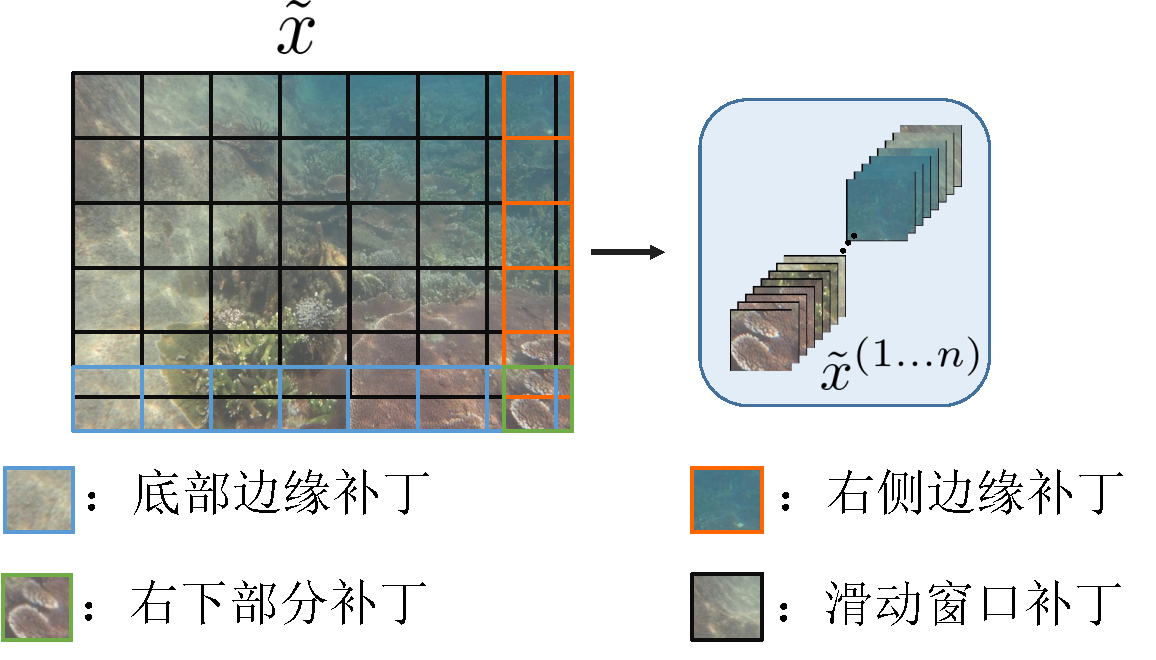
\includegraphics[width=0.8\textwidth]{figures/ch3/patch.pdf}
    \caption{水下退化图像的补丁分解示例(在滑动窗口步长$s$等于补丁大小$p$时,除边缘区域外,补丁不重叠)。}
    \label{img:patch}
\end{figure}


\subsection{基于条件去噪的采样过程}

条件扩散模型在生成任务中表现出卓越的性能,被广泛应用于图像编辑和恢复任务\cite{cDDPM} \cite{rst_DDPM}。
本章利用条件扩散模型的基本原理将退化的水下图像作为条件信息引入扩散模型采样过程中,从而确保生成结果的保真度和对目标图像特性的精确还原。
\begin{figure}
    \centering
    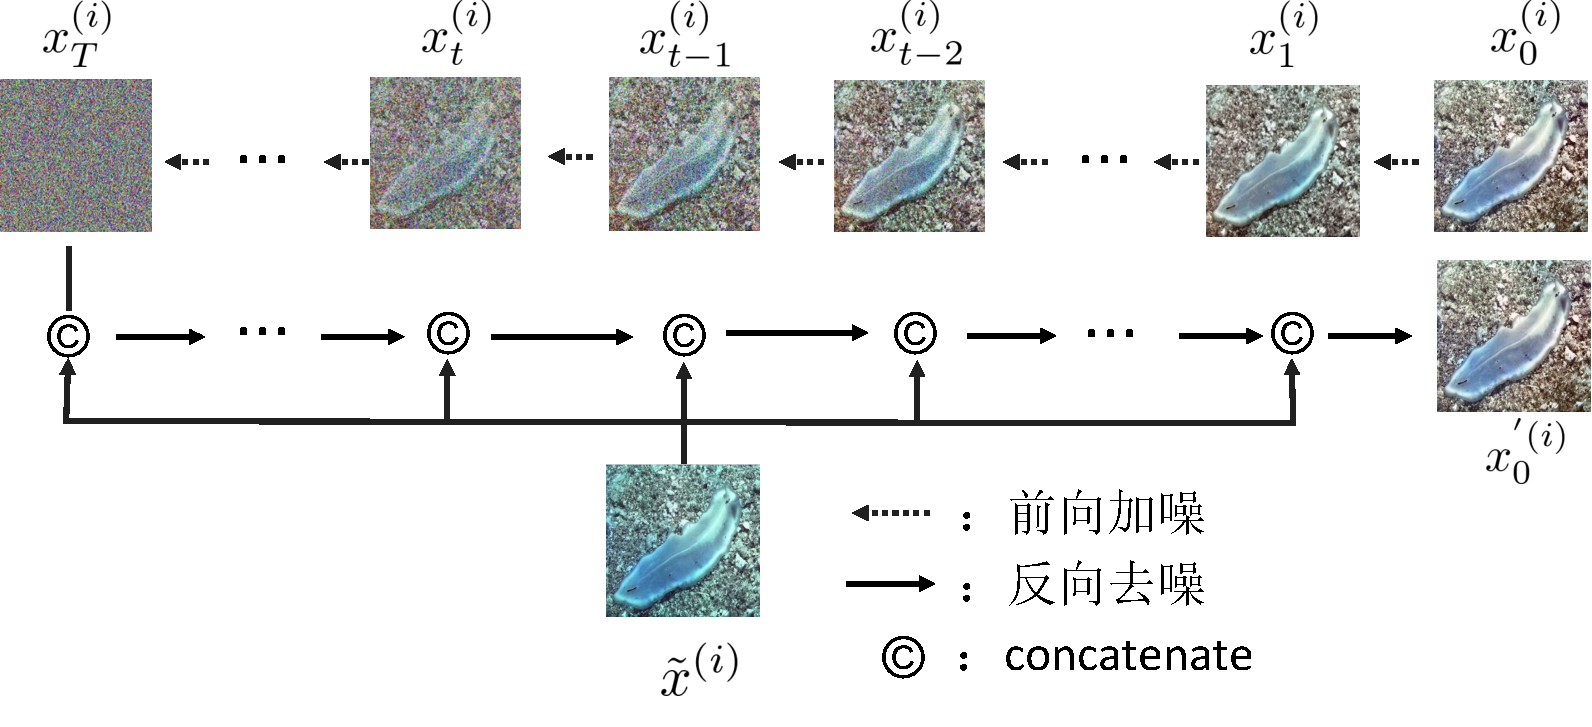
\includegraphics[width=0.8\textwidth]{figures/ch3/cond_ddpm.pdf}
    \caption{基于条件去噪的采样过程示意图。}
    \label{img:cond_ddpm}
\end{figure}

如图 \ref{img:cond_ddpm} 所示,在采样过程中,模型将退化的水下图像补丁 $\tilde{\mathbf{x}}^{(i)}$ 与当前时间步的输入噪声补丁 $\mathbf{x}^{(i)}_t$ 在通道维度上进行拼接,
生成一个六通道的组合图像。该组合图像随后被输入到噪声估计网络中,以学习条件下的噪声分布。
这一设计能够有效地结合输入噪声与退化图像信息,指导模型生成具有高保真度的去噪图像。

如算法 \ref{alg:training} 所示,训练过程中首先确定一幅完整图像的所有补丁位置掩码 $\bm{P}$,
然后随机选择一个补丁编号 $i$,以获取对应的水下清晰图像补丁 $\mathbf{x}_0^{(i)}$ 和退化的条件图像补丁 $\tilde{\mathbf{x}}^{(i)}$。
这种随机选择策略有效增加了训练数据的多样性,并降低了模型对特定补丁位置的过拟合风险。

在每次迭代中,执行以下步骤:
(1)从时间步集合 $T$ 中随机采样一个时间步长$t \sim \text{Uniform}\{1,\ldots,T\}$。
(2)从标准正态分布中生成噪声 $\bm{\epsilon}_t \sim \mathcal{N}(\mathbf{0}, \mathbf{I})$。
(3)根据公式\eqref{eq:x0_xt_patch},将噪声添加到清晰补丁 $\mathbf{x}_0^{(i)}$:
\begin{equation}
\label{eq:x0_xt_patch}
    \mathbf{x}_t^{(i)} = \sqrt{\bar{\alpha}_t} \mathbf{x}_0^{(i)} + \sqrt{1 - \bar{\alpha}_t} \bm{\epsilon}_t
\end{equation}

利用梯度下降算法训练的核心是优化模型参数 $\theta$,使其能够准确预测噪声 $\bm{\epsilon}_\theta$。目标是最小化以下损失函数:
\begin{equation}
    \nabla_{\theta}\vert\vert\bm{\epsilon}_t -  \bm{\epsilon}_{\theta}(\sqrt{\bar{\alpha}_t}\mathbf{x}_0^{(i)}+\sqrt{1-\bar{\alpha}_t}\bm{\epsilon}_t\,,\tilde{\mathbf{x}}^{(i)},t)\vert\vert^2
\end{equation}

\begin{algorithm}[ht]
    \SetAlgoLined
    \KwIn{干净图像 $\bm{X}_0$ 和退化图像 $\bm{\tilde{X}}$}
    \KwOut{训练后的模型参数 $\theta$}
  
    $n \leftarrow P.\text{length}$\;
    \Repeat{收敛}{
      随机采样一个补丁ID $i \in \{1, 2, 3, \ldots, n\}$,来自不同的补丁位置\;
      $\mathbf{x}_0^{(i)} \leftarrow \text{Crop}(\bm{P}_i \circ \bm{X}_0)$\;
      $\tilde{\mathbf{x}}^{(i)} \leftarrow \text{Crop}(\bm{P}_i \circ \bm{\tilde{X}})$\;
      $t \sim \text{Uniform}\{1, \ldots, T\}$ 且 $\bm{\epsilon}_t \sim \mathcal{N}(\mathbf{0}, \mathbf{I})$\;
      对以下目标执行一次梯度下降步骤:\\
      \quad $\nabla_{\theta} \Vert \bm{\epsilon}_t - \bm{\epsilon}_{\theta}(\sqrt{\bar{\alpha}_t}\mathbf{x}_0^{(i)} + \sqrt{1 - \bar{\alpha}_t}\bm{\epsilon}_t, \tilde{\mathbf{x}}^{(i)}, t) \Vert^2$\;
    }
    \caption{训练}
    \label{alg:training}
  \end{algorithm}

如算法 \ref{alg:inference} 所示,采样过程中将退化的水下图像 $\tilde{\bm{X}}$ 作为条件信息,为模型提供参考。
采样图像 $\bm{X}_t$ 的初始状态为标准正态分布随机噪声:$\bm{X}_t \sim \mathcal{N}(\mathbf{0}, \mathbf{I})$。
在每个时间步 $s$ 中,通过退化图像补丁的指导,逐步去除噪声,生成最终清晰图像 $\bm{X}_t$。

% 对于基于补丁的DDIM采样器来说,其后向采样公式\eqref{eq:p}更新为:
% \begin{equation}
% \begin{split}
%     \label{eq:ddim}
%      \mathbf{x}^{(i)}_{t-1} =& \sqrt{\bar{\alpha}_{t-1}}\left(\frac{\mathbf{x}^{(i)}_t-\sqrt{1-\bar{\alpha}_t} \cdot \boldsymbol{\epsilon}_\theta\left(\mathbf{x}^{(i)}_t, t\right)}{\sqrt{\bar{\alpha}_t}}\right) \\
%      + &\sqrt{1-\bar{\alpha}_{t-1}} \cdot \epsilon_\theta\left(\mathbf{x}^{(i)}_t, t\right)
% \end{split}
% \end{equation}

对于采样过程,如果将采样步骤数设置为 $S$,每个时间步对应一个噪声去除阶段 $t$ 和 $t_{\text{next}}$,采样过程的主要步骤如下:
(1)首先从 $n$ 个补丁掩码列表 $P$ 中,提取当前图像补丁 $\mathbf{x}_t^{(i)}$ 和条件补丁 $\tilde{\mathbf{x}}^{(i)}$。
使用训练好的噪声估计网络 $\bm{\epsilon}_\theta$,为每个补丁单独预测当前时间步的噪声补丁 $\bm{\epsilon}_\theta\left(\mathbf{x}_t^{(i)}, \tilde{\mathbf{x}}^{(i)}, t\right)$;
(2)将每个补丁的噪声预测值累加到全局噪声估计矩阵 $\bm{\hat{\epsilon}}_t$,同时更新权重矩阵 $\mathbf{M}$,用于记录每个像素的累计权重;
(3)使用逐元素除法计算全局平均噪声估计:$\bm{\hat{\epsilon}}_t \leftarrow \bm{\hat{\epsilon}}_t \oslash \mathbf{M}$;
(4)最后根据估计的全局噪声 $\bm{\hat{\epsilon}}_t$,按照公式\eqref{eq:x0_xt}更新当前时间步的图像 $\bm{X}t$。
重复上述步骤直至所有时间步 $S$ 完成,最终返回清晰图像 $\bm{X}_t$,如算法\ref{alg:inference}所示。
\begin{algorithm}[ht]
    \SetAlgoLined
    \KwIn{退化图像 $\tilde{\bm{X}}$,隐式采样时间步数 $S$}
    \KwOut{采样后的图像 $\bm{X}_t$}
  
    $\bm{X}_{t} \sim \mathcal{N}(\mathbf{0}, \mathbf{I})$\;
    \For{$s = S,\ldots,1$}{
      $t \leftarrow (s-1) \cdot T / S + 1$\;
      \eIf{$s > 1$}{
        $t_{\text{next}} \leftarrow (s-2) \cdot T / S + 1$\;
      }{
        $t_{\text{next}} \leftarrow 0$\;
      }
      $\bm{\hat{\epsilon}}_t \leftarrow \mathbf{0}$\;
      $\mathbf{M} \leftarrow \mathbf{0}$\;
      \For{$i = 1,\ldots,n$}{
        $\mathbf{x}_t^{(i)} \leftarrow \text{Crop}(\mathbf{P}_i \circ \bm{X}_t)$\;
        $\tilde{\mathbf{x}}^{(i)} \leftarrow \text{Crop}(\mathbf{P}_i \circ \tilde{\bm{X}})$\;
        $\bm{\hat{\epsilon}}_t \leftarrow \bm{\hat{\epsilon}}_t + \mathbf{P}_i \cdot \bm{\epsilon}_{\theta}(\mathbf{x}_t^{(i)}, \tilde{\mathbf{x}}^{(i)}, t)$\;
        $\mathbf{M} \leftarrow \mathbf{M} + \mathbf{P}_i$\;
      }
      $\bm{\hat{\epsilon}}_t \leftarrow \bm{\hat{\epsilon}}_t \oslash \mathbf{M}$ \quad \quad $\oslash$: 元素级除法\;
      $X_{t} \leftarrow \sqrt{\bar{\alpha}_{t_{\text{next}}}} \left(\frac{X_t - \sqrt{1 - \bar{\alpha}_t} \cdot \bm{\hat{\epsilon}}_t}{\sqrt{\bar{\alpha}_t}}\right) + \sqrt{1 - \bar{\alpha}_{t_{\text{next}}}} \cdot \bm{\hat{\epsilon}}_t$\;
    }
    \Return $\bm{X}_t$\;
    \caption{采样}
    \label{alg:inference}
  \end{algorithm}

\section{噪声估计网络结构}
目前去噪扩散模型的噪声估计网络大多基于 U-Net \cite{unet}架构,
本章分别通过修改和引入残差模块和注意力机制,设计了一种针对图像补丁的噪声估计网络。

如图 \ref{img:network} 所示,噪声估计网络采用带有跳跃连接的编码器-解码器架构,其输入为当前时间步 $t$ 的图像补丁 $\mathbf{x}^{(i)}_t$ 和对应的条件补丁 $\tilde{\mathbf{x}}^{(i)}$拼接形成的六通道数据。经过初始卷积操作后,输入被送入编码器进行特征提取,结果解码器生成预测的结果$\boldsymbol{\epsilon}_\theta(\mathbf{x}_t, t)$。
\begin{figure}[ht]
    \centering 
    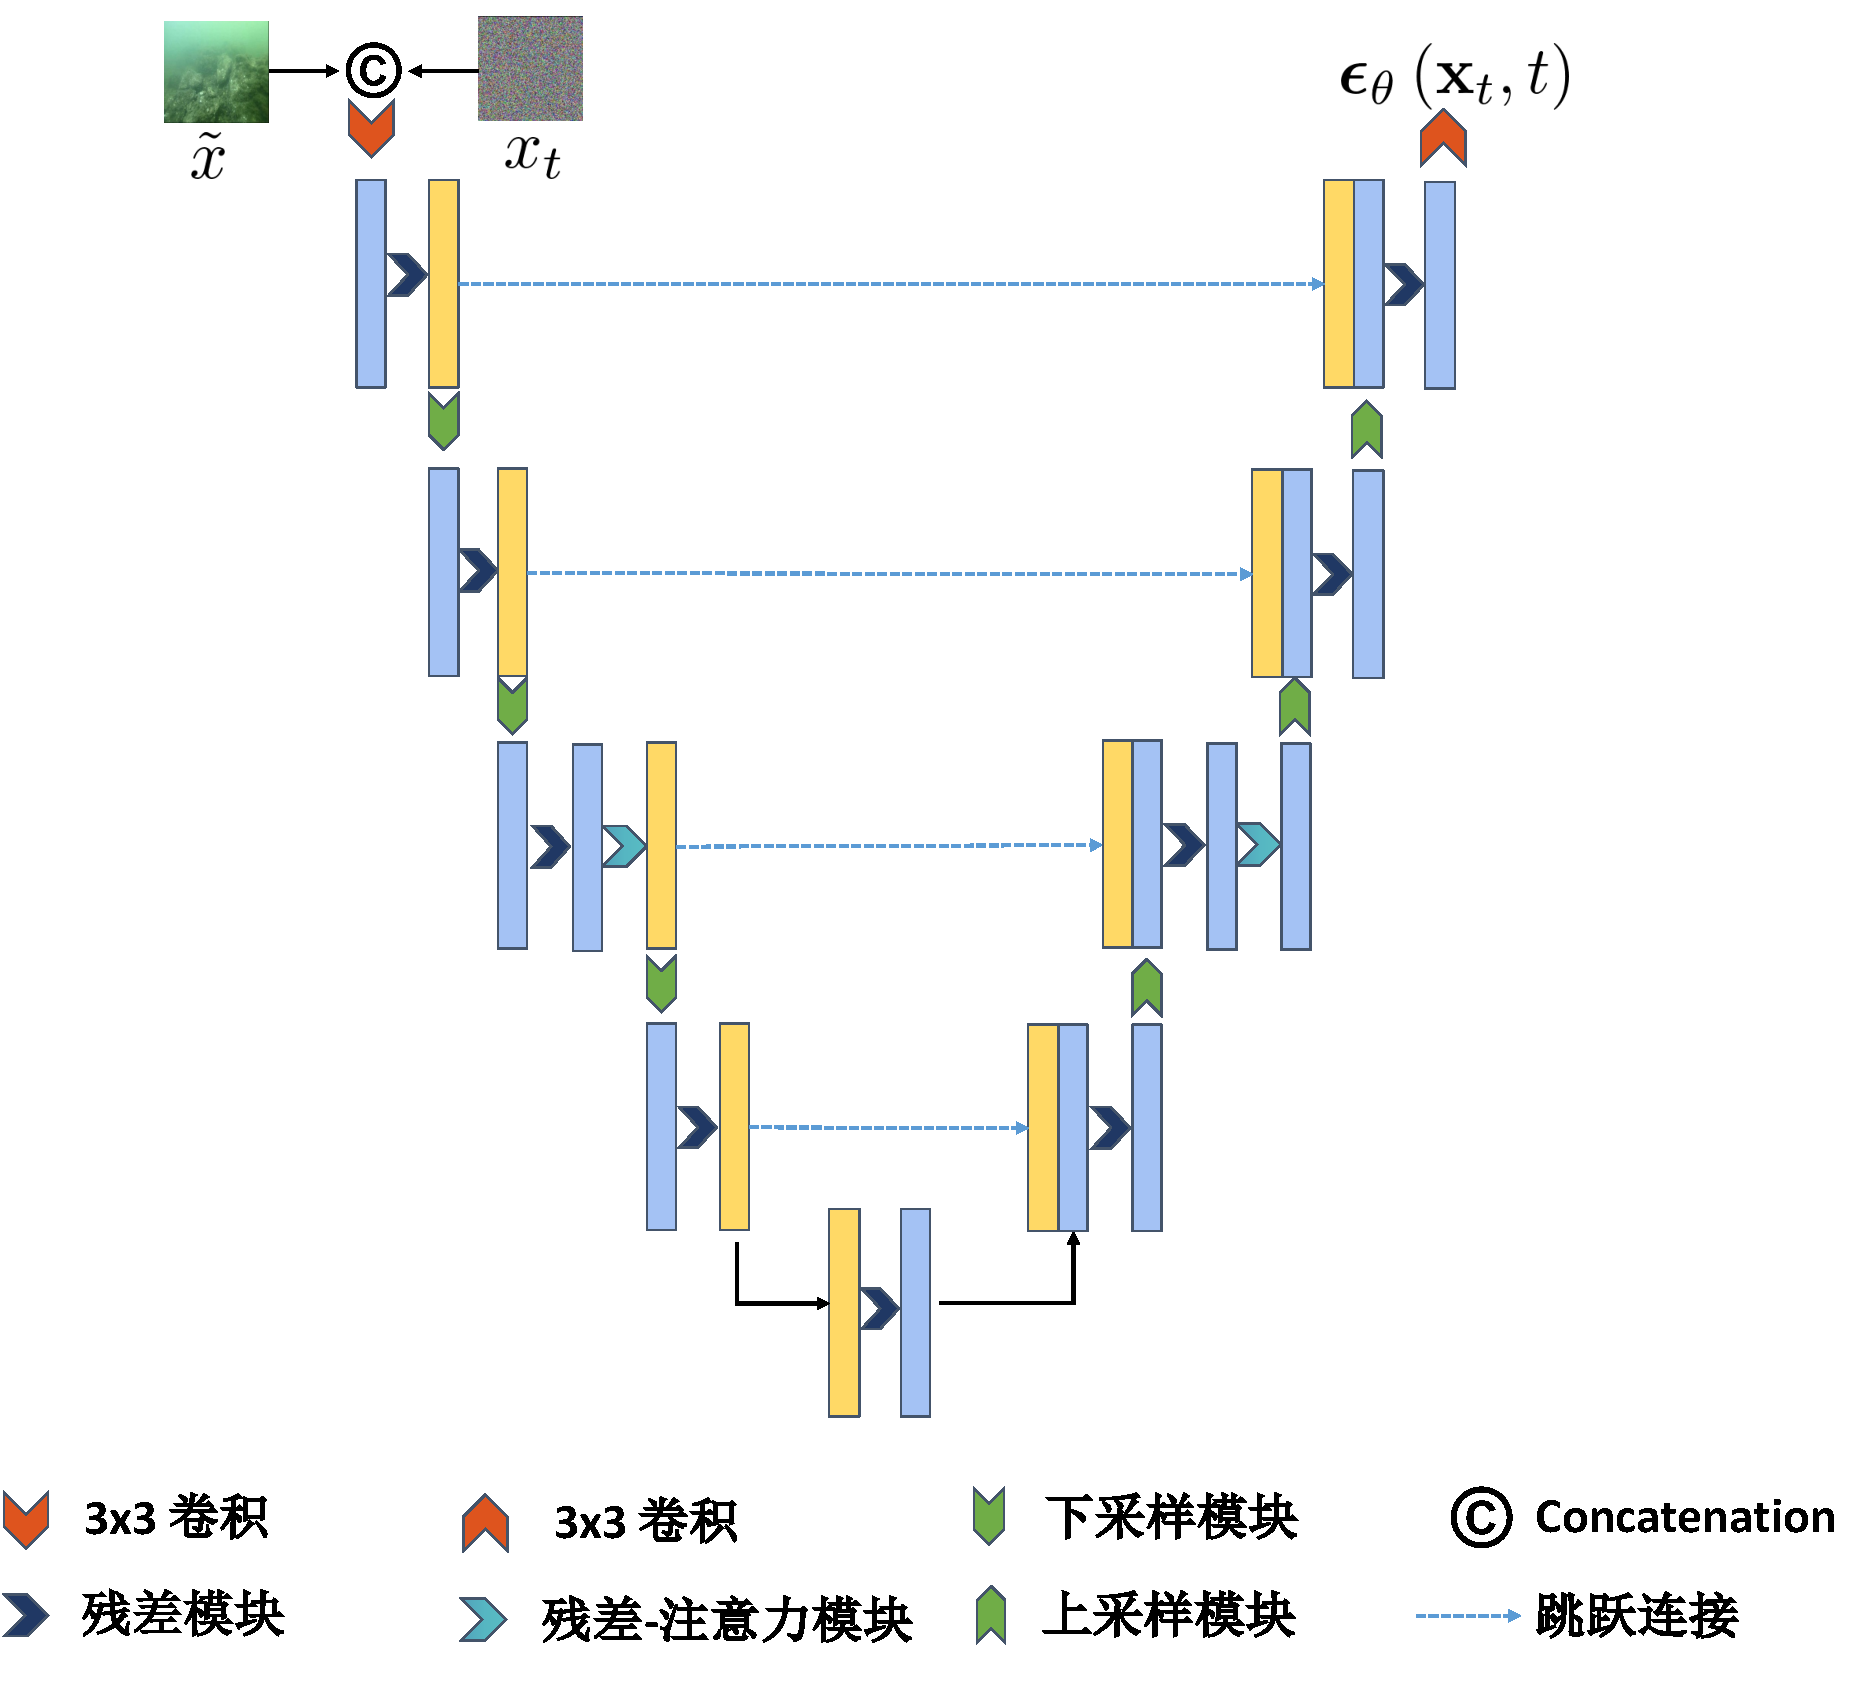
\includegraphics[width=0.8\textwidth]{figures/ch3/network.pdf}
    \caption{去噪生成网络结构示意图。}
    \label{img:network}
\end{figure}

\subsection{残差模块的特征处理}
特征处理是深度学习模型中提升特征表达能力的重要步骤,尤其是在复杂任务中,深层次的特征处理可以有效提高模型的学习能力。
残差网络(ResNet)\cite{resnet}在特征处理任务中发挥了重要作用。通过引入跨层残差连接,ResNet 缓解了深层网络中的梯度消失问题,并显著提升了特征提取的效率和精度。
本章设计的残差模块在ResNet基础上,添加了时间步的嵌入信息,如\ref{img:module}所示:
在每个残差模块中都加入一个经过正弦-余弦位置编码(sin-cos positional encoding)处理的时间步嵌入信息,
该嵌入信息经过全连接层后,与上一层的特征融合,提供时间步的相关性支持。
在卷积操作之前,模块依次执行组归一化(Group Normalization)、非线性激活函数(ReLU)和 Dropout 操作。
卷积操作后的输出会与前一层输入结合,实现跨层的残差连接。
这种设计既提升了特征的表达能力,又通过残差路径有效缓解了梯度消失问题,使模型能够更深层次地学习复杂特征。

\subsection{残差注意力模块的深度融合}
注意力机制是近年来深度学习中广泛应用的一种方法,通过捕捉特征中的全局依赖关系,显著增强了模型对关键特征的表达能力。
在本章中,我们引入了残差-注意力模块(Residual-Attention Module)以进一步提升模型的特征提取能力,
尤其是在编码器和解码器中特定分辨率为 $16 \times 16$ 的层中(如图\ref{img:network})。残差注意力模块详细设计如下:
如图\ref{img:module}所示,首先对上一层输入特征进行组归一化,确保特征分布的一致性,
再经过自注意力机制捕捉输入特征中不同位置之间的全局依赖关系,
之后将经过自注意力处理的特征输入一个 $1 \times 1$ 的卷积层,用作残差连接的Shortcut层。
最后通过残差连接,将卷积层的输出与原始输入特征融合。

类似于 Transformer 中的注意力机制 \cite{2017attention},通过引入残差路径,模块不仅增强了全局特征的感知能力,还避免了深层网络中的梯度消失问题。
残差-注意力模块的引入使模型能够在局部卷积之外关注更广范围的特征关系。特别是在处理复杂图像结构或需要全局特征分析时,该模块展现出了显著优势。
结合编码器和解码器的联合作用,模型能够更加准确地估计噪声,生成高质量的结果。

\subsection{可学习的采样策略}
编码器的核心任务是逐步压缩输入特征的空间分辨率,以提取高层次特征并为解码阶段提供丰富的语义信息。
如图 \ref{img:module} 所示,本章设计的编码器中的下采样并未采用传统的池化操作,而是用步长为 2 的卷积操作代替。这种设计使下采样过程成为一个可学习的阶段,使网络能够自主优化特征压缩方式,从而更加灵活地适应输入数据的特点。

解码器通过逐步上采样还原特征的空间分辨率,最终输出预测的噪声估计结果 $\boldsymbol{\epsilon}_\theta(\mathbf{x}_t, t)$。
上采样操作的实现方式主要包括两种:(1)线性插值结合卷积:通过插值扩展特征图尺寸,然后使用卷积操作进一步优化特征。(2)反卷积:直接通过反卷积操作增加特征的空间分辨率。
如图 \ref{img:module} 所示,本章选择了反卷积方式进行上采样,
通过反卷积操作从瓶颈层的低分辨率特征图逐步还原到输入图像的原始尺寸。
相比插值结合卷积的方式,反卷积具有更强的学习能力,能够动态调整特征映射的还原方式。

此外,类似-Net的设计,解码器中通过四次跳跃连接(Skip Connections),将编码器中对应分辨率的特征直接传递到解码器,弥补了下采样过程中可能丢失的信息。
这种设计显著提高了生成结果的质量和一致性。算法整体采样过程如图\ref{img:sample_process}所示。
\begin{figure}[ht]
    \centering
    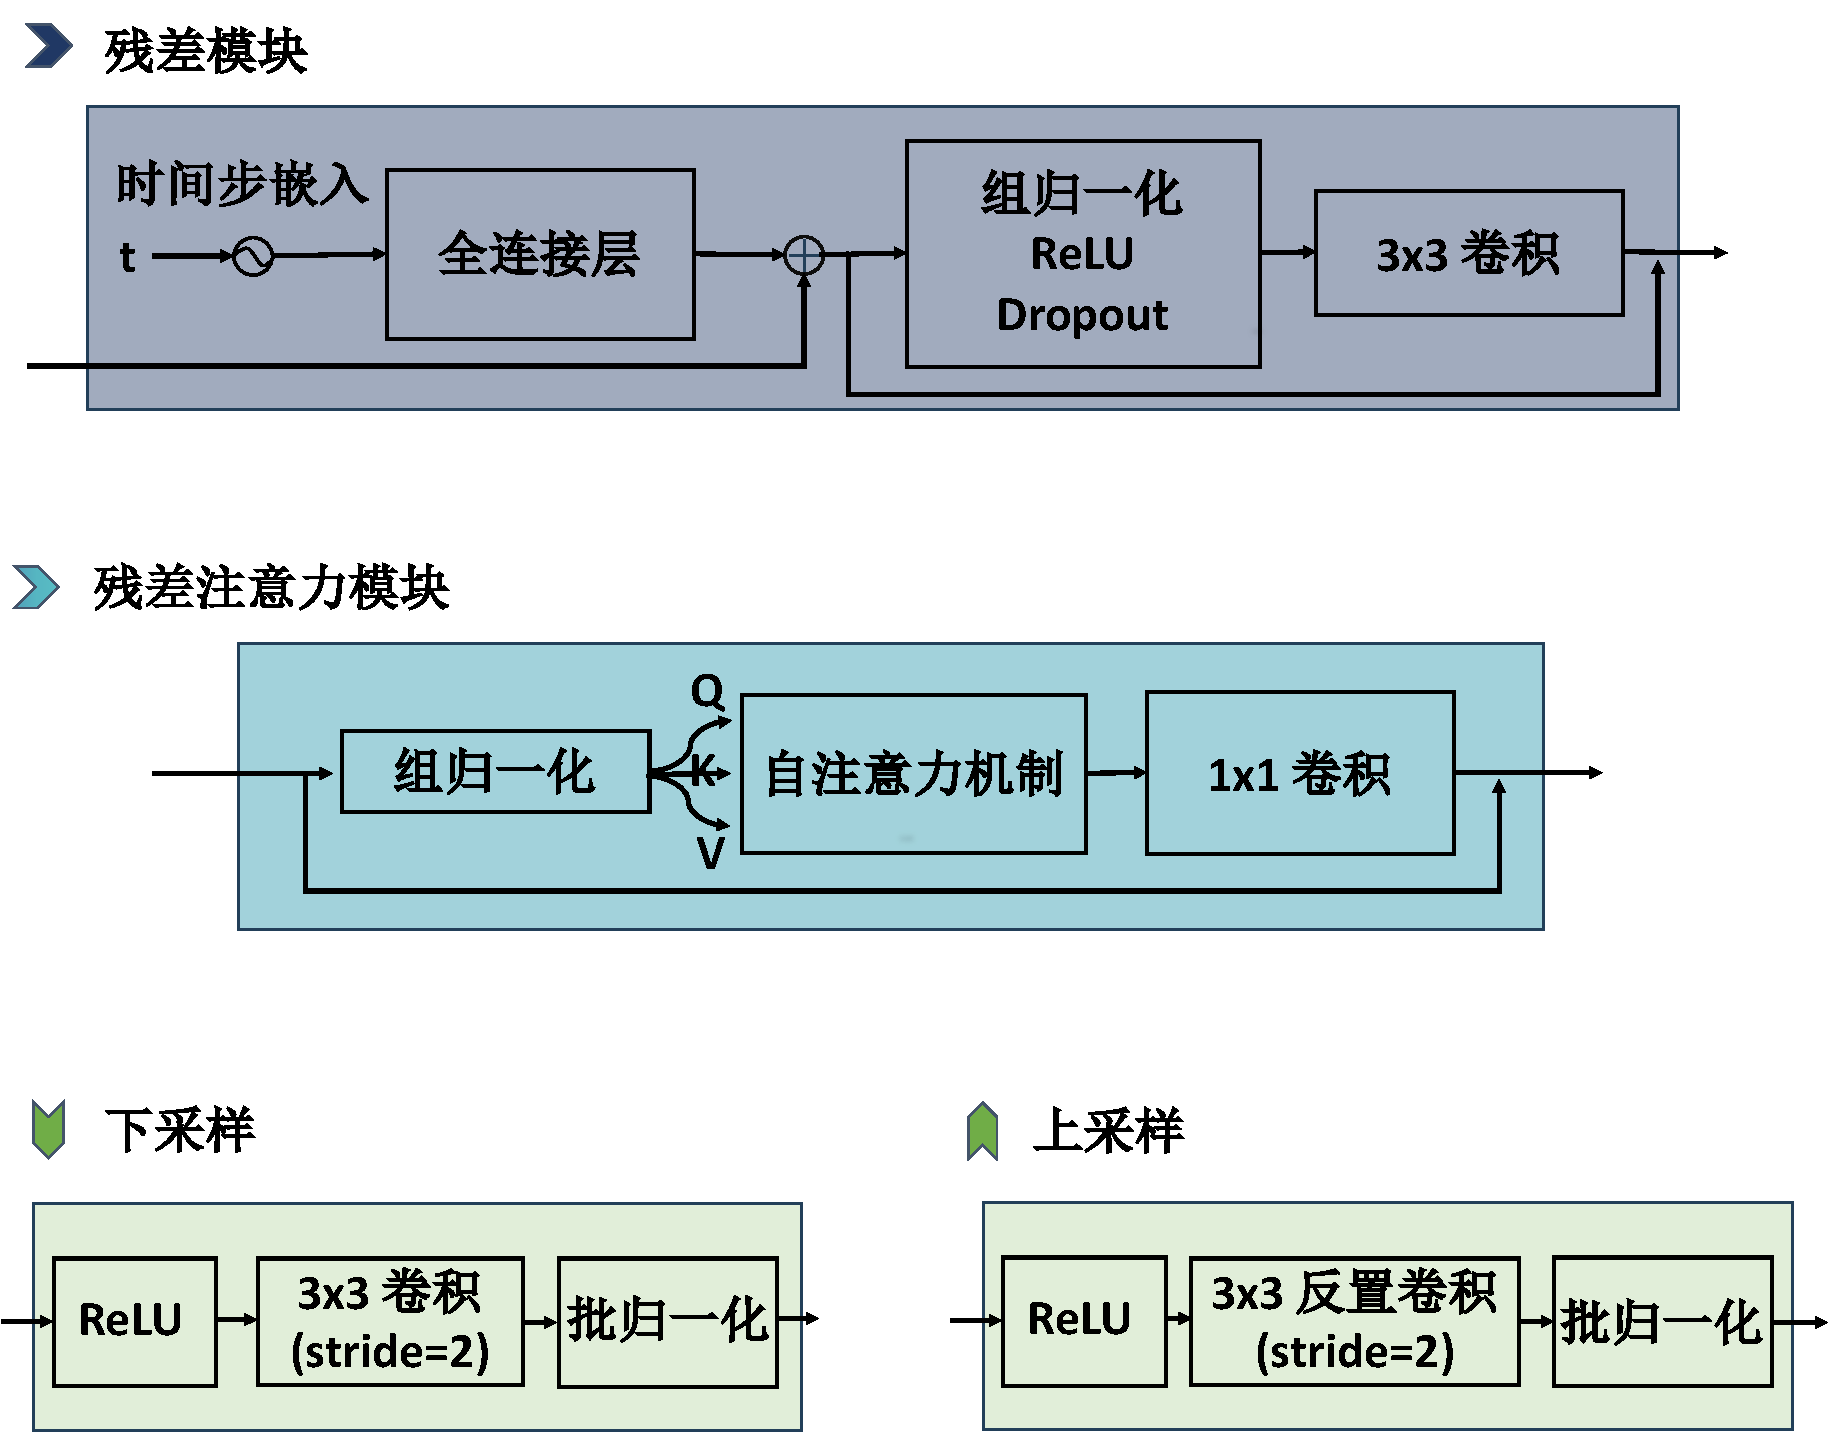
\includegraphics[width=0.8\textwidth]{figures/ch3/module.pdf}
    \caption{各模块示意图。}
    \label{img:module}
    \vspace{0.4cm}
\end{figure}

\begin{figure}[ht]
    \centering
    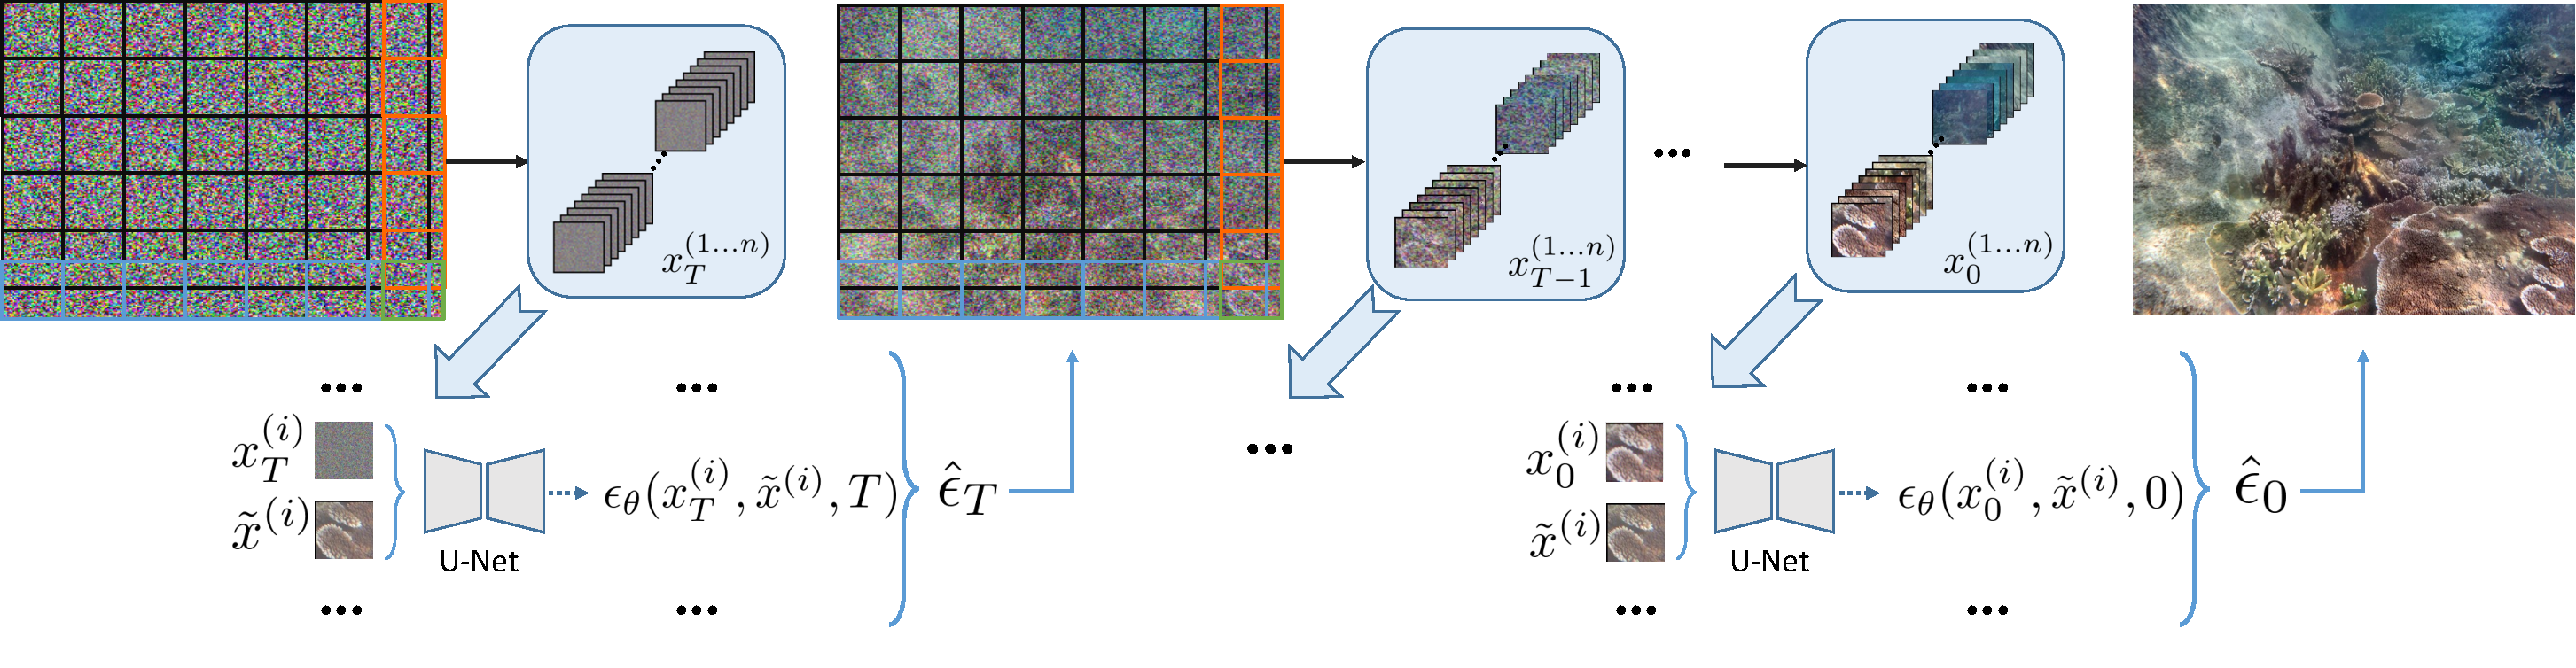
\includegraphics[width=0.98\textwidth]{figures/ch3/sample_process.pdf}
    \caption{各模块示意图。}
    \label{img:sample_process}
\end{figure} 


\section{实验结果与分析}
\subsection{实验设置}
实验选用了两个开源的水下图像增强数据集——EUVP \cite{funie_gan} 和 UIEB \cite{uieb} 作为基准数据集,
其中EUVP 数据集包含 11,435 对配对的水下图像,涵盖三种不同的风格,图像分辨率主要为 $256 \times 256$,
UIEB 数据集包含 890 对配对图像以及 60 张无参考图像。
该数据集的分辨率相比EUVP较高,图 \ref{img:scatter} 展示了两个数据集分辨率的分布情况。
训练集和测试集的划分见表 \ref{tab:dataset-split}。
\begin{figure}[ht]
    \centering
    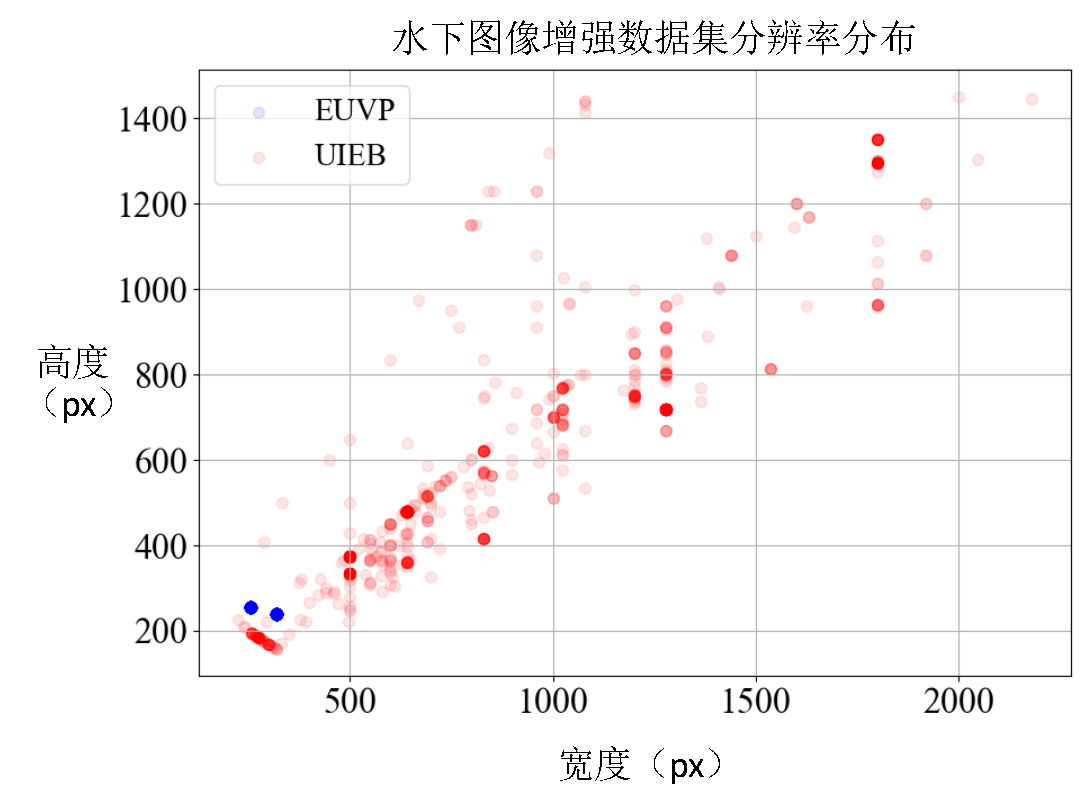
\includegraphics[width=0.8\textwidth]{figures/ch3/scatter.pdf}
    \caption{EUVP 和 UIEB 数据集中图像的分辨率分布。}
    \label{img:scatter}
\end{figure}

\begin{table}[ht]
	\vspace{-0.4mm}
	\centering
	\caption{\label{tab:dataset-split}数据集划分(成对图像)。}
	\vspace{-2mm}
	\setlength{\tabcolsep}{2.6mm}{
		\begin{tabular}{lccc}
			\toprule
			\specialrule{0em}{1pt}{1pt}
			\textbf{数据集}  & \textbf{训练集}  & \textbf{测试集} & \textbf{共计} \\
			\hline
			\specialrule{0em}{1pt}{1pt}
			EUVP (paired) \cite{funie_gan}  & $8,363$  & $3,072$  & $11,435$\\
			\specialrule{0em}{1pt}{1pt}
                UIEB (paired) \cite{uieb}  & $678$  & $212$  & $890$\\
			\bottomrule
	\end{tabular}}
	\vspace{-1mm}
\end{table}   

实验基于 PyTorch 框架,在 NVIDIA RTX3060 GPU 上进行。
整个训练过程迭代 500,000 次,批量大小为 8。图像补丁大小设置为 $64 \times 64$,与噪声估计网络的输入维度一致。
优化器采用 Adam \cite{kingma2017adam},学习率为 $2 \times 10^{-4}$。

去噪扩散模型采样过程的总采样步数 $T$ 设置为 1000,基于去噪扩散隐式模型的采样推理步数 $S$ 设置为 20,以加速推理。
方差调度参数 $\beta_i$ 采用线性变化,从 0.0001 逐步增加到 0.02。

\subsection{定量评价}
水下图像增强评估选用三种常见的水下图像质量评价指标,用于不同方法的水下图像增强效果进行定量比较,具体包括:

(1)峰值信噪比(PSNR):用于评估参考图像和增强图像之间的像素重建质量,计算公式如下:
\begin{equation}
    \mathrm{PSNR} =10 \times \log _{10} \frac{(\mathrm{MAXI})^2}{\mathrm{MSE}}
\end{equation}

其中,$\mathrm{MAXI}$ 表示像素值的动态范围,$\mathrm{MSE}$ 表示参考图像和增强图像之间的均方误差。

(2)结构相似性指数(SSIM) \cite{ssim}:从亮度、对比度和结构三个方面评价图像之间的相似性,计算公式如下:
\begin{equation}
    \mathrm{SSIM} = \frac{{(2\mu_x\mu_y + c_1)(2\sigma_{xy} + c_2)}}{{(\mu_x^2 + \mu_y^2 + c_1)(\sigma_x^2 + \sigma_y^2 + c_2)}}
\end{equation}

其中,$\mu_x$、$\mu_y$ 表示参考图像和重建图像的均值,$\sigma_x^2、\sigma_y^2$ 表示方差,$\sigma_{xy}$ 表示协方差,$c_1=(255\times0.01)^2$、$c_2=(255\times0.03)^2$ 是稳定因子。

(3)水下图像质量指标(UIQM) \cite{uiqm}:一种无参考质量指标,结合了水下图像的色彩、清晰度和对比度特性,计算公式如下:
\begin{equation}
    \mathrm{UIQM}=c_1 \times \mathrm{UICM}+c_2 \times \mathrm{UISM}+c_3 \times \mathrm{UIConM}
\end{equation}

其中,$\mathrm{UICM}$、$\mathrm{UISM}$ 和 $\mathrm{UIConM}$ 分别用来衡量水下图像的色彩、锐度和对比度,$c1=0.0282$、$c2=0.2953$、$c3=3.5753$为权重系数。

表\ref{tab:psnr-ssim}  和表\ref{tab:uiqm} 分别展示了本章提出的水下图像增强的方法与其他方法在 PSNR、SSIM 和 UIQM 等指标上的比较结果。
其中 Ucolor\cite{ucolor}模型需要额外的传输图作为输入,
由于DCP系列方法可以生成额外的传输图,并且本章的实验包括UDCP\cite{udcp}算法,所以使用UDCP生成的传输图来评估Ucolor模型,
而Ucolor所提出的原始方法使用一般暗通道\cite{GDCP}提取所需的传输图。
实验结果表明本章提出的水下图像增强方法在多个指标上表现优越,
在有参考质量指标(PSNR 和 SSIM)方面展现了具有接近高质量参考图像水平,
在无参考指标(UIQM)上,基于去噪扩散模型的水下图像增强方法的综合表现仍处于领先地位,在提升增强图像的细节质量与全局一致性方面具有明显优势。

\begin{table*}[t]
	\footnotesize
        \captionsetup{justification=centering}
	\caption{不同方法在数据集 EUVP 和 UIEB 上的 PSNR 和 SSIM 定量结果。以红色字体显示的分数代表该行中排名最高的方法。}
	\label{tab:psnr-ssim}
	\vspace{-0.4mm}
	\centering
	\setlength{\tabcolsep}{1.01mm}{
		\renewcommand{\arraystretch}{1.1}
            \begin{tabular}{cccccccccc}
			\toprule
			数据集 & 指标 & UDCP\cite{udcp} & UGAN\cite{ugan} & FGAN\cite{funie_gan} & UWCNN\cite{uwcnn} & Ucolor\cite{ucolor} & STSC\cite{stsc} & U-shape\cite{u-shape} & Ours\\
			\hline
			\multirow{2}{*}{EUVP} & \textbf{PSNR} & $16.71$ & $27.46$ & $26.59$ & $21.56$ & $26.27$ & $20.71$ & $26.23$ & $\textcolor{red}{\textbf{30.29}}$ \\ & \textbf{SSIM} & $0.76$ & $0.87$ & $0.84$ & $0.84$ & $0.89$ & $0.83$ & $0.88$ & $\textcolor{red}{\textbf{0.92}}$ \\
            \vspace{-2mm} 
             \hspace*{\fill} \\
			% \hline
            
			\multirow{2}{*}{UIEB} & \textbf{PSNR} & $13.20$ & $21.01$ & $20.76$ & $14.86$ & $\textcolor{red}{\textbf{23.90}}$ & $21.46$ & $20.94$ & $21.34$ \\ & \textbf{SSIM}  & $0.70$ & $0.69$ & $0.68$ & $0.69$ & $0.91$ & $0.72$ & $0.62$ & $\textcolor{red}{\textbf{0.92}}$  \\
			\bottomrule
	\end{tabular}}
	\vspace{-0.4mm}
\end{table*}   % paired

\begin{table*}[t]
	%	\vspace{-4mm}
	\footnotesize
	\caption{不同方法在数据集 EUVP 和 UIEB 上的 UIQM 定量结果。以红色字体显示的分数代表该行中排名最高的方法。}
	\label{tab:uiqm}
	\vspace{-0.4mm}
	\centering
	\setlength{\tabcolsep}{1.01mm}{
		\renewcommand{\arraystretch}{1.1}
		% \begin{tabular}{c|c|ccccccc|c}
            \begin{tabular}{cccccccccc}
			\toprule
			数据集 & 指标 & UDCP\cite{udcp} & UGAN\cite{ugan} & FGAN\cite{funie_gan} & UWCNN\cite{uwcnn} & Ucolor\cite{ucolor} & STSC\cite{stsc} & U-shape\cite{u-shape} & Ours\\
			\hline
			\multirow{4}{*}{EUVP} & UICM & $\textcolor{red}{\textbf{5.85}}$ & $3.76$ & $4.54$ & $2.97$ & $3.94$ &  $5.31$ & $4.16$ & $4.67$ \\
			& UISM & $6.28$ & $7.40$ & $7.15$ & $6.85$ & $7.33$ & $\textcolor{red}{\textbf{7.41}}$ & $7.29$ & $7.25$\\
                & UIConM & $0.03$ & $0.22$ & $0.20$ & $0.29$ & $0.27$ &
            $0.28$ & $0.27$ & $\textcolor{red}{\textbf{0.30}}$\\
                 % \cline{2-10}
                & \textbf{UIQM} & $2.13$ & $3.08$ & $2.97$ & $3.15$ & $3.25$ &
            $3.34$ & $3.22$ & $\textcolor{red}{\textbf{3.35}}$ \\
            \vspace{-2mm} 
             \hspace*{\fill} \\
			% \hline
			\multirow{4}{*}{UIEB} & UICM & $\textcolor{red}{\textbf{6.70}}$ & $5.63$ & $5.44$ & $2.69$ & $5.06$ & $5.80$ & $4.91$ & $5.28$ \\
			& UISM & $5.42$ & $5.35$ & $5.24$ & $4.98$ & $6.74$ & $5.25$ & $5.32$ & $\textcolor{red}{\textbf{7.08}}$\\
                & UIConM & $0.04$ & $0.29$ & $0.29$ & $0.31$ & $0.30$ &
            $\textcolor{red}{\textbf{0.33}}$ & $0.32$ & $0.30$\\
                % \cline{2-10}
                & \textbf{UIQM} & $1.97$ & $2.77$ & $2.74$ & $2.65$ & $3.20$ &
            $2.89$ & $2.86$ & $\textcolor{red}{\textbf{3.32}}$\\
			\bottomrule
	\end{tabular}}
	\vspace{-0.4mm}
\end{table*}   

\subsection{主观评价}
如图\ref{img:scatter} 展示的 EUVP 和 UIEB 数据集中图像的分辨率分布,基准数据集中的图像分辨率大小并不一致,
而大多数基于深度学习的水下图像增强方法(如 FGAN\cite{funie_gan}、UGAN\cite{ugan}、U-shape\cite{u-shape} 和 STSC\cite{stsc})
均在固定的输入和输出尺寸下进行训练和推理。而本章方法具备更高的分辨率适应性。

如图\ref{img:visual-euvp}和图\ref{img:visual-uieb}所示,首先在$256 \times 256$ 图像分辨率尺寸下实验对比了不同方法在 EUVP 和 UIEB 数据集上的主观增强效果。
实验结果表明,本章提出的水下图像增强方法在保持图像真实感的同时,显著提升了水下物体的色彩表现。
尤其在蓝色和绿色主导的水域场景中,可以增强画面色彩饱和度和自然感。
\begin{figure}[t]
	\begin{center}
		\begin{tabular}{ccccccccc}
			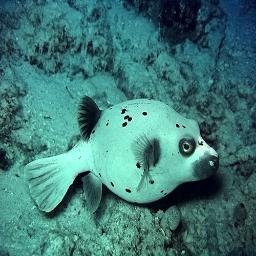
\includegraphics[width = 0.10\linewidth,height=0.10\linewidth]{figures/ch3/compare/EUVP/Input/264318_n02655020_17544.JPEG} & \hspace{-0.40cm}
			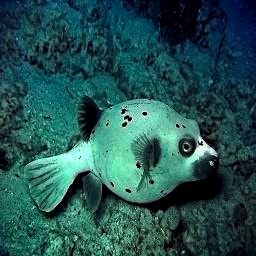
\includegraphics[width = 0.10\linewidth,height=0.10\linewidth]{figures/ch3/compare/EUVP/UDCP/264318_n02655020_17544.JPEG}  & \hspace{-0.40cm}
			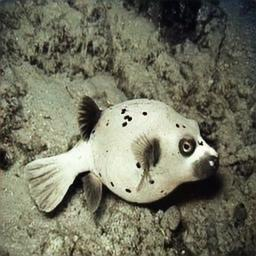
\includegraphics[width = 0.10\linewidth,height=0.10\linewidth]{figures/ch3/compare/EUVP/UGAN/264318_n02655020_17544.JPEG}  & \hspace{-0.40cm}
			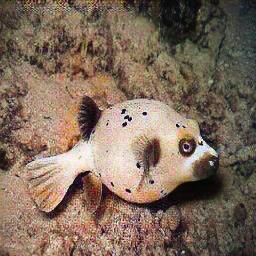
\includegraphics[width = 0.10\linewidth,height=0.10\linewidth]{figures/ch3/compare/EUVP/FGAN/264318_n02655020_17544.JPEG}  & \hspace{-0.40cm}
			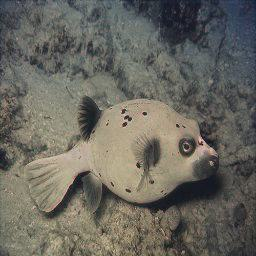
\includegraphics[width = 0.10\linewidth,height=0.10\linewidth]{figures/ch3/compare/EUVP/UWCNN/264318_n02655020_17544.JPEG} & \hspace{-0.40cm}
			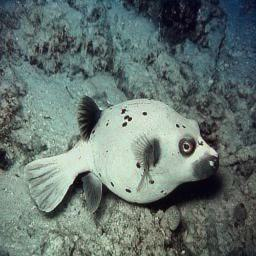
\includegraphics[width = 0.10\linewidth,height=0.10\linewidth]{figures/ch3/compare/EUVP/Ucolor/264318_n02655020_17544.JPEG}& \hspace{-0.40cm}
			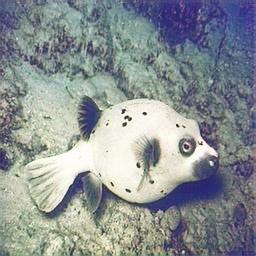
\includegraphics[width = 0.10\linewidth,height=0.10\linewidth]{figures/ch3/compare/EUVP/STSC/264318_n02655020_17544.JPEG}  & \hspace{-0.40cm}
			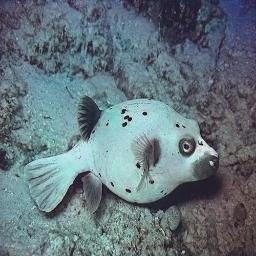
\includegraphics[width = 0.10\linewidth,height=0.10\linewidth]{figures/ch3/compare/EUVP/Ushape/264318_n02655020_17544.JPEG}& \hspace{-0.40cm} 
            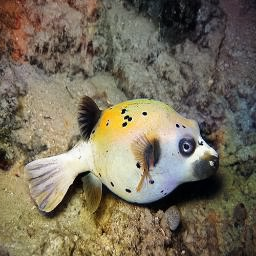
\includegraphics[width = 0.10\linewidth,height=0.10\linewidth]{figures/ch3/compare/EUVP/Ours/264318_n02655020_17544..png}  \\
                
            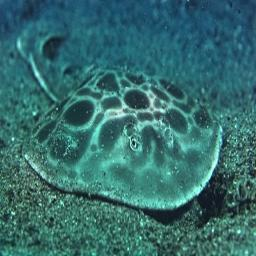
\includegraphics[width = 0.10\linewidth,height=0.10\linewidth]{figures/ch3/compare/EUVP/Input/265613_n01496331_8134.JPEG}  & \hspace{-0.40cm}
			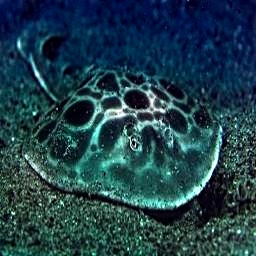
\includegraphics[width = 0.10\linewidth,height=0.10\linewidth]{figures/ch3/compare/EUVP/UDCP/265613_n01496331_8134.JPEG}   & \hspace{-0.40cm}
			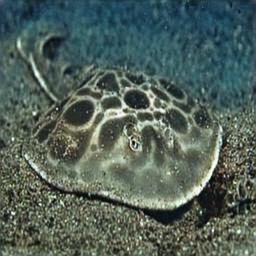
\includegraphics[width = 0.10\linewidth,height=0.10\linewidth]{figures/ch3/compare/EUVP/UGAN/265613_n01496331_8134.JPEG}   & \hspace{-0.40cm}
			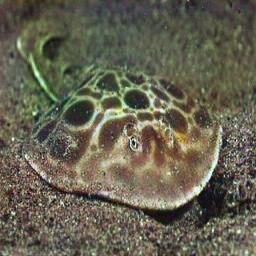
\includegraphics[width = 0.10\linewidth,height=0.10\linewidth]{figures/ch3/compare/EUVP/FGAN/265613_n01496331_8134.JPEG}   & \hspace{-0.40cm}
			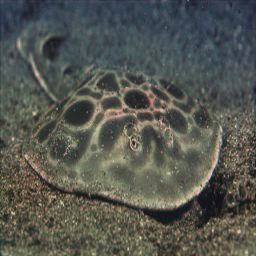
\includegraphics[width = 0.10\linewidth,height=0.10\linewidth]{figures/ch3/compare/EUVP/UWCNN/265613_n01496331_8134.JPEG}  & \hspace{-0.40cm}
			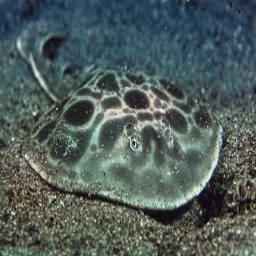
\includegraphics[width = 0.10\linewidth,height=0.10\linewidth]{figures/ch3/compare/EUVP/Ucolor/265613_n01496331_8134.JPEG} & \hspace{-0.40cm}
			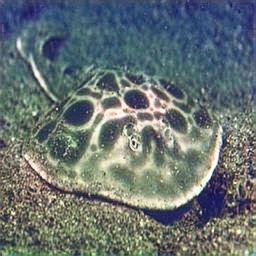
\includegraphics[width = 0.10\linewidth,height=0.10\linewidth]{figures/ch3/compare/EUVP/STSC/265613_n01496331_8134.JPEG}   & \hspace{-0.40cm}
			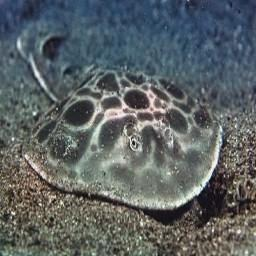
\includegraphics[width = 0.10\linewidth,height=0.10\linewidth]{figures/ch3/compare/EUVP/Ushape/265613_n01496331_8134.JPEG} & \hspace{-0.40cm}         
			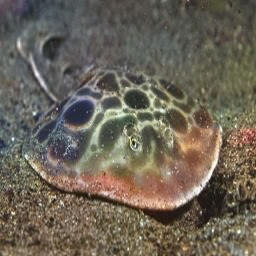
\includegraphics[width = 0.10\linewidth,height=0.10\linewidth]{figures/ch3/compare/EUVP/Ours/265613_n01496331_8134..png}   \\

            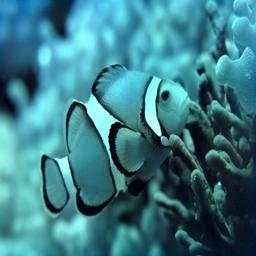
\includegraphics[width = 0.10\linewidth,height=0.10\linewidth]{figures/ch3/compare/EUVP/Input/264298_00035269.jpg}  & \hspace{-0.40cm}
			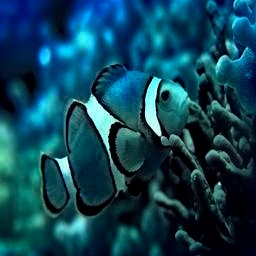
\includegraphics[width = 0.10\linewidth,height=0.10\linewidth]{figures/ch3/compare/EUVP/UDCP/264298_00035269.jpg}   & \hspace{-0.40cm}
			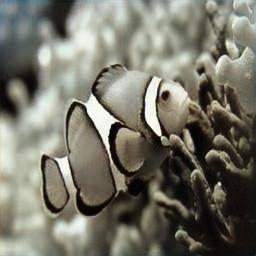
\includegraphics[width = 0.10\linewidth,height=0.10\linewidth]{figures/ch3/compare/EUVP/UGAN/264298_00035269.jpg}   & \hspace{-0.40cm}
			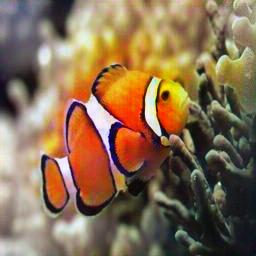
\includegraphics[width = 0.10\linewidth,height=0.10\linewidth]{figures/ch3/compare/EUVP/FGAN/264298_00035269.jpg}   & \hspace{-0.40cm}
			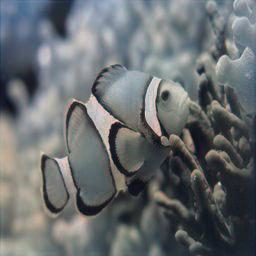
\includegraphics[width = 0.10\linewidth,height=0.10\linewidth]{figures/ch3/compare/EUVP/UWCNN/264298_00035269.jpg}  & \hspace{-0.40cm}
			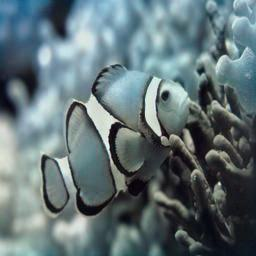
\includegraphics[width = 0.10\linewidth,height=0.10\linewidth]{figures/ch3/compare/EUVP/Ucolor/264298_00035269.jpg} & \hspace{-0.40cm}
			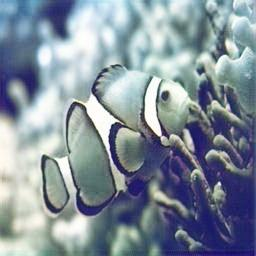
\includegraphics[width = 0.10\linewidth,height=0.10\linewidth]{figures/ch3/compare/EUVP/STSC/264298_00035269.jpg}   & \hspace{-0.40cm}
			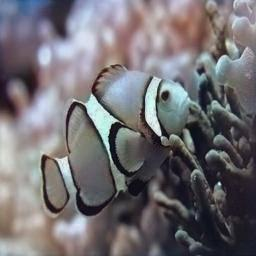
\includegraphics[width = 0.10\linewidth,height=0.10\linewidth]{figures/ch3/compare/EUVP/Ushape/264298_00035269.jpg} & \hspace{-0.40cm}         
			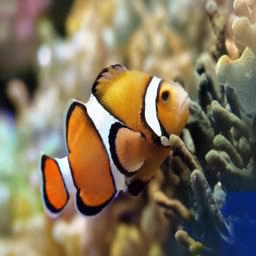
\includegraphics[width = 0.10\linewidth,height=0.10\linewidth]{figures/ch3/compare/EUVP/Ours/264298_00035269.png}   \\

            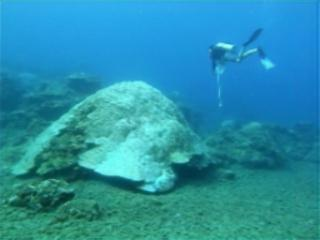
\includegraphics[width = 0.10\linewidth,height=0.10\linewidth]{figures/ch3/compare/EUVP/Input/im_f149_.jpg}  & \hspace{-0.40cm}
			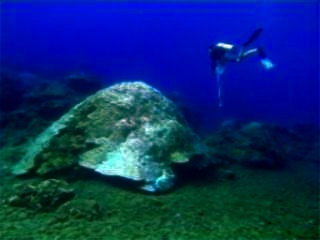
\includegraphics[width = 0.10\linewidth,height=0.10\linewidth]{figures/ch3/compare/EUVP/UDCP/im_f149_.jpg}   & \hspace{-0.40cm}
			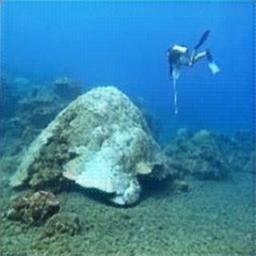
\includegraphics[width = 0.10\linewidth,height=0.10\linewidth]{figures/ch3/compare/EUVP/UGAN/im_f149_.jpg}   & \hspace{-0.40cm}
			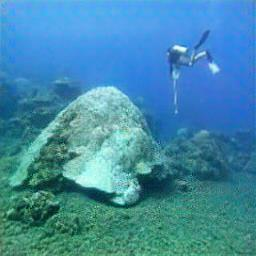
\includegraphics[width = 0.10\linewidth,height=0.10\linewidth]{figures/ch3/compare/EUVP/FGAN/im_f149_.jpg}   & \hspace{-0.40cm}
			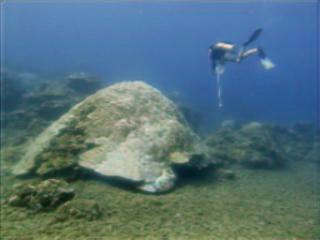
\includegraphics[width = 0.10\linewidth,height=0.10\linewidth]{figures/ch3/compare/EUVP/UWCNN/im_f149_.jpg}  & \hspace{-0.40cm}
			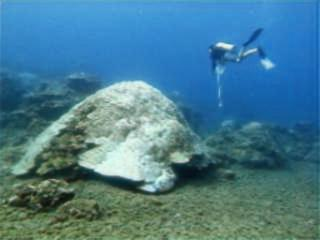
\includegraphics[width = 0.10\linewidth,height=0.10\linewidth]{figures/ch3/compare/EUVP/Ucolor/im_f149_.jpg} & \hspace{-0.40cm}
			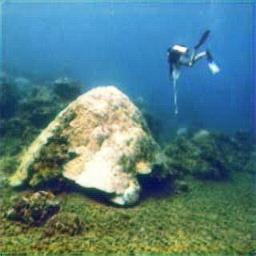
\includegraphics[width = 0.10\linewidth,height=0.10\linewidth]{figures/ch3/compare/EUVP/STSC/im_f149_.jpg}   & \hspace{-0.40cm}
			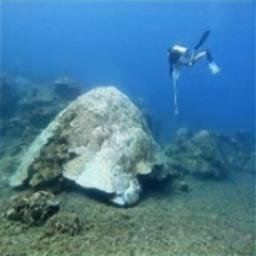
\includegraphics[width = 0.10\linewidth,height=0.10\linewidth]{figures/ch3/compare/EUVP/Ushape/im_f149_.jpg} & \hspace{-0.40cm}  
			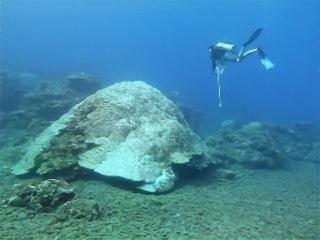
\includegraphics[width = 0.10\linewidth,height=0.10\linewidth]{figures/ch3/compare/EUVP/Ours/im_f149_.png}   
            \\
			\scriptsize Input
			&\hspace{-0.50cm} \scriptsize UDCP\cite{udcp}
			&\hspace{-0.50cm} \scriptsize UGAN\cite{ugan}
			&\hspace{-0.50cm} \scriptsize FGAN\cite{funie_gan}
			&\hspace{-0.50cm} \scriptsize UWCNN\cite{uwcnn}
			&\hspace{-0.50cm} \scriptsize Ucolor\cite{ucolor}
			&\hspace{-0.50cm} \scriptsize STSC\cite{stsc}
			&\hspace{-0.50cm} \scriptsize U-shape\cite{u-shape}
			&\hspace{-0.50cm} \scriptsize Ours
			\\

		\end{tabular}
	\end{center}
	\vspace{-0.4mm}
	\caption{\label{img:visual-euvp}EUVP 数据集上的主观结果比较。在大多数情况下,本章的方法相比其他方法能够更好地恢复物体的颜色,提升画面色彩和对比度。}
	\vspace{-0.3mm}
\end{figure} 

\begin{figure*}[t]
    \vspace{-1mm}
\begin{center}
    \begin{tabular}{ccccccccc}
        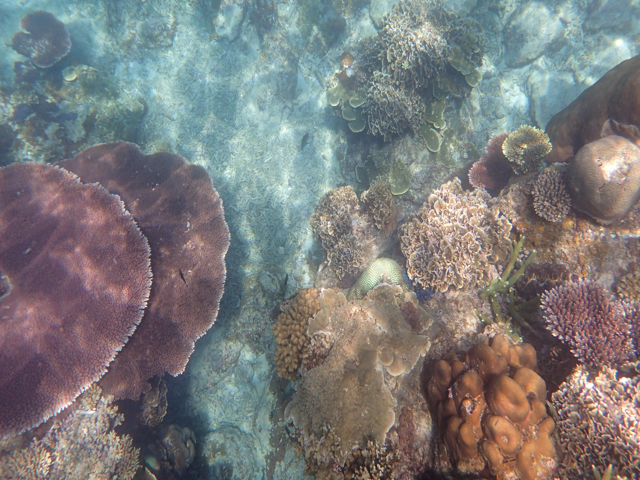
\includegraphics[width = 0.10\linewidth,height=0.10\linewidth]{figures/ch3/compare/UIEB/Input/161_img_.png} & \hspace{-0.40cm}
        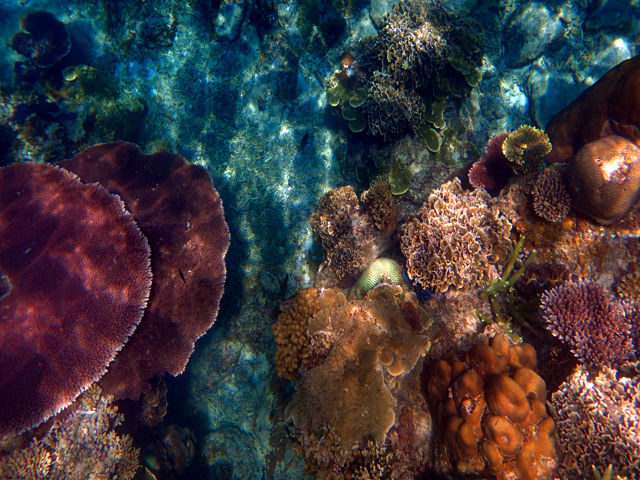
\includegraphics[width = 0.10\linewidth,height=0.10\linewidth]{figures/ch3/compare/UIEB/UDCP/161_img_.png}  & \hspace{-0.40cm}
        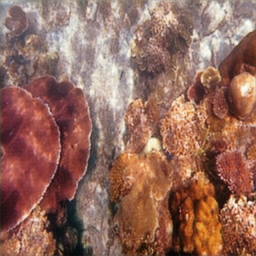
\includegraphics[width = 0.10\linewidth,height=0.10\linewidth]{figures/ch3/compare/UIEB/UGAN/161_img_.png}  & \hspace{-0.40cm}
        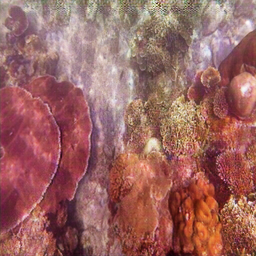
\includegraphics[width = 0.10\linewidth,height=0.10\linewidth]{figures/ch3/compare/UIEB/FGAN/161_img_.png}  & \hspace{-0.40cm}
        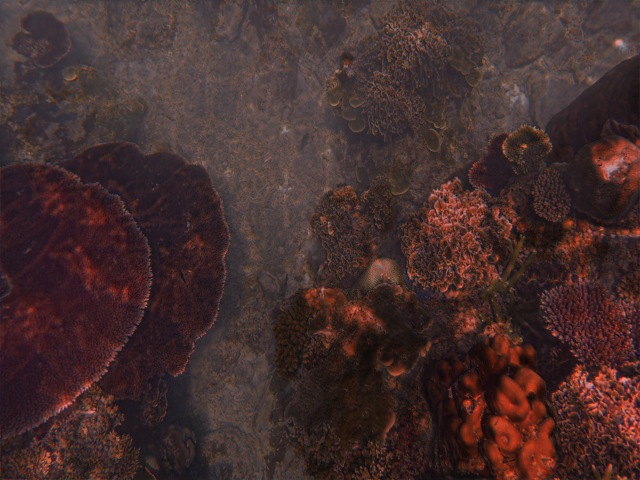
\includegraphics[width = 0.10\linewidth,height=0.10\linewidth]{figures/ch3/compare/UIEB/UWCNN/161_img_.png} & \hspace{-0.40cm}
        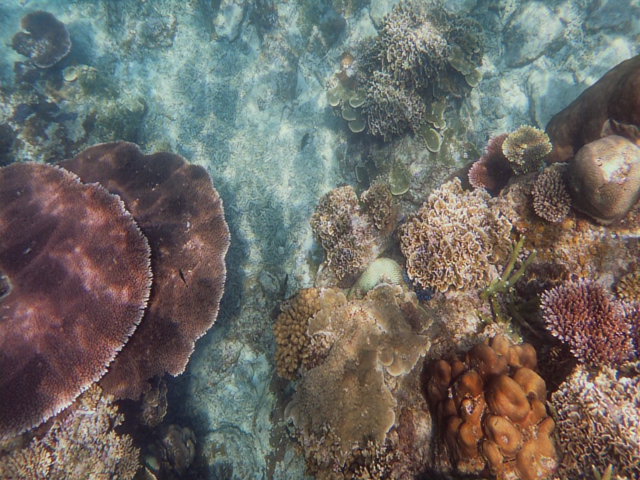
\includegraphics[width = 0.10\linewidth,height=0.10\linewidth]{figures/ch3/compare/UIEB/Ucolor/161_img_.png}& \hspace{-0.40cm}
        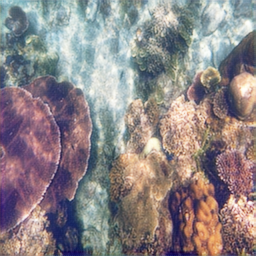
\includegraphics[width = 0.10\linewidth,height=0.10\linewidth]{figures/ch3/compare/UIEB/STSC/161_img_.png}  & \hspace{-0.40cm}
        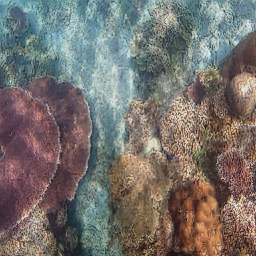
\includegraphics[width = 0.10\linewidth,height=0.10\linewidth]{figures/ch3/compare/UIEB/Ushape/161_img_.png}& \hspace{-0.40cm} 
        \includegraphics[width = 0.10\linewidth,height=0.10\linewidth]{figures/ch3/compare/UIEB/Ours/161_img_.png}  \\

        \includegraphics[width = 0.10\linewidth,height=0.10\linewidth]{figures/ch3/compare/UIEB/Input/41_img_.png} & \hspace{-0.40cm}
        \includegraphics[width = 0.10\linewidth,height=0.10\linewidth]{figures/ch3/compare/UIEB/UDCP/41_img_.png}  & \hspace{-0.40cm}
        \includegraphics[width = 0.10\linewidth,height=0.10\linewidth]{figures/ch3/compare/UIEB/UGAN/41_img_.png}  & \hspace{-0.40cm}
        \includegraphics[width = 0.10\linewidth,height=0.10\linewidth]{figures/ch3/compare/UIEB/FGAN/41_img_.png}  & \hspace{-0.40cm}
        \includegraphics[width = 0.10\linewidth,height=0.10\linewidth]{figures/ch3/compare/UIEB/UWCNN/41_img_.png} & \hspace{-0.40cm}
        \includegraphics[width = 0.10\linewidth,height=0.10\linewidth]{figures/ch3/compare/UIEB/Ucolor/41_img_.png}& \hspace{-0.40cm}
        \includegraphics[width = 0.10\linewidth,height=0.10\linewidth]{figures/ch3/compare/UIEB/STSC/41_img_.png}  & \hspace{-0.40cm}
        \includegraphics[width = 0.10\linewidth,height=0.10\linewidth]{figures/ch3/compare/UIEB/Ushape/41_img_.png}& \hspace{-0.40cm} 
        \includegraphics[width = 0.10\linewidth,height=0.10\linewidth]{figures/ch3/compare/UIEB/Ours/41_img_.png} 
        \\
        \scriptsize Input
        & \hspace{-0.51cm} \scriptsize UDCP\cite{udcp}
        & \hspace{-0.51cm} \scriptsize UGAN*\cite{ugan}
        & \hspace{-0.51cm} \scriptsize FGAN*\cite{funie_gan}
        & \hspace{-0.51cm} \scriptsize UWCNN\cite{uwcnn}
        & \hspace{-0.51cm} \scriptsize Ucolor\cite{ucolor}
        & \hspace{-0.51cm} \scriptsize STSC*\cite{stsc}
        & \hspace{-0.51cm} \scriptsize U-shape*\cite{u-shape}
        & \hspace{-0.51cm} \scriptsize Ours
        \\
    \end{tabular}
\end{center}
\vspace{-1mm}
\caption{\label{img:visual-uieb}UIEB 数据集上的主观结果比较。本章的方法在高分辨率图像上依旧保持良好的色彩校正能力。(标注为 “*” 的方法限制图像分辨率为 $256 \times 256$)。}
\vspace{-1mm}
\end{figure*}

实验进一步分析了不同方法在高分辨率图像上的增强效果(如图 \ref{img:visual-detail} 所示),
与需要对图像进行压缩处理的方法(FGAN\cite{funie_gan}、UGAN\cite{ugan}、U-shape\cite{u-shape} 和 STSC\cite{stsc})对比,
本章提出的水下图像增强方法可以在不损失图像细节的情况下对任意分辨率的水下图像进行有效增强,在保留物体表面的细节纹理的同时增强色彩和对比度。

\begin{figure}[ht]
	\begin{center}
        \includegraphics[width=0.96\linewidth]{figures/ch3/compare/discussion/res_detail.jpg}
		\\
        \setlength{\tabcolsep}{0pt} % 默认通常是6pt
        \begin{tabular}{
            >{\centering\arraybackslash}p{0.16\linewidth}
            >{\centering\arraybackslash}p{0.16\linewidth}
            >{\centering\arraybackslash}p{0.16\linewidth}
            >{\centering\arraybackslash}p{0.16\linewidth}
            >{\centering\arraybackslash}p{0.16\linewidth}
            >{\centering\arraybackslash}p{0.16\linewidth}
        }
            \footnotesize Input \hspace{-1.5cm}
			& \footnotesize FGAN\cite{funie_gan} 
			& \footnotesize UGAN\cite{ugan} 
			& \footnotesize STSC\cite{stsc} 
			& \footnotesize U-shape\cite{u-shape} 
			& \footnotesize Ours
            \\ 
		\end{tabular}
	\end{center}
	\caption{ \label{img:visual-detail}UIEB 数据集中不同分辨率图像的增强结果比较。对于存在输入大小限制的四种模型使用线性插值来调整其结果的图像分辨率。}
	\vspace{-2mm}
\end{figure}

% \begin{figure}[ht]
% 	\begin{center}
% 		\begin{tabular}{c c c c c c}
% 			\includegraphics[width = 0.15\linewidth]{figures/ch3/compare/resolution/input/2_img__merged.png} & \hspace{-0.50cm}
% 			\includegraphics[width = 0.15\linewidth]{figures/ch3/compare/resolution/FGAN/2_img__resize_merged.png}  & \hspace{-0.50cm}
% 			\includegraphics[width = 0.15\linewidth]{figures/ch3/compare/resolution/UGAN/2_img__resize_merged.png}  & \hspace{-0.50cm}
% 			\includegraphics[width = 0.15\linewidth]{figures/ch3/compare/resolution/STSC/2_img__resize_merged.png}  & \hspace{-0.50cm}
%             \includegraphics[width = 0.15\linewidth]{figures/ch3/compare/resolution/Ushape/2_img__resize_merged.png}  & \hspace{-0.50cm}
% 			\includegraphics[width = 0.15\linewidth]{figures/ch3/compare/resolution/ours/2_img__merged.png}  \\

%             \includegraphics[width = 0.15\linewidth]{figures/ch3/compare/resolution/input/19_img__merged.png} & \hspace{-0.50cm}
% 			\includegraphics[width = 0.15\linewidth]{figures/ch3/compare/resolution/FGAN/19_img__resize_merged.png}  & \hspace{-0.50cm}
% 			\includegraphics[width = 0.15\linewidth]{figures/ch3/compare/resolution/UGAN/19_img__resize_merged.png}  & \hspace{-0.50cm}
% 			\includegraphics[width = 0.15\linewidth]{figures/ch3/compare/resolution/STSC/19_img__resize_merged.png}  & \hspace{-0.50cm}
%             \includegraphics[width = 0.15\linewidth]{figures/ch3/compare/resolution/Ushape/19_img__resize_merged.png}  & \hspace{-0.50cm}
% 			\includegraphics[width = 0.15\linewidth]{figures/ch3/compare/resolution/ours/19_img__merged.png}  \\

%             \includegraphics[width = 0.15\linewidth]{figures/ch3/compare/resolution/input/129_img__merged.png} & \hspace{-0.50cm}
% 			\includegraphics[width = 0.15\linewidth]{figures/ch3/compare/resolution/FGAN/129_img__resize_merged.png}  & \hspace{-0.50cm}
% 			\includegraphics[width = 0.15\linewidth]{figures/ch3/compare/resolution/UGAN/129_img__resize_merged.png}  & \hspace{-0.50cm}
% 			\includegraphics[width = 0.15\linewidth]{figures/ch3/compare/resolution/STSC/129_img__resize_merged.png}  & \hspace{-0.50cm}
%             \includegraphics[width = 0.15\linewidth]{figures/ch3/compare/resolution/Ushape/129_img__resize_merged.png}  & \hspace{-0.50cm}
% 			\includegraphics[width = 0.15\linewidth]{figures/ch3/compare/resolution/ours/129_img__merged.png}  \\

%             \includegraphics[width = 0.15\linewidth]{figures/ch3/compare/resolution/input/17_img__merged.png} & \hspace{-0.50cm}
% 			\includegraphics[width = 0.15\linewidth]{figures/ch3/compare/resolution/FGAN/17_img__resize_merged.png}  & \hspace{-0.50cm}
% 			\includegraphics[width = 0.15\linewidth]{figures/ch3/compare/resolution/UGAN/17_img__resize_merged.png}  & \hspace{-0.50cm}
% 			\includegraphics[width = 0.15\linewidth]{figures/ch3/compare/resolution/STSC/17_img__resize_merged.png}  & \hspace{-0.50cm}
%             \includegraphics[width = 0.15\linewidth]{figures/ch3/compare/resolution/Ushape/17_img__resize_merged.png}  & \hspace{-0.50cm}
% 			\includegraphics[width = 0.15\linewidth]{figures/ch3/compare/resolution/ours/17_img__merged.png}  
%             \\  
% 			\footnotesize Input
% 			& \hspace{-0.36cm} \footnotesize FGAN\cite{funie_gan}
% 			& \hspace{-0.36cm} \footnotesize UGAN\cite{ugan}
% 			& \hspace{-0.36cm} \footnotesize STSC\cite{stsc}
% 			& \hspace{-0.36cm} \footnotesize U-shape\cite{u-shape}
%             & \hspace{-0.36cm} \footnotesize Ours
% 			\\
% 		\end{tabular}
% 	\end{center}
% 	\vspace{-3mm}
% 	\caption{ \label{img:visual-detail}The detailed comparison of enhancement results of four images from the UIEB datasets at different resolutions. We use linear interpolation to resize the image resolution of the results obtained from the other four models.}
% 	\vspace{-3mm}
% \end{figure} 


\subsection{结果讨论}
\subsubsection{水下语义恢复}
为了验证本章提出的水下图像增强算法在减轻水下环境对语义干扰上的有效性,
采用显著性区域检测网络 \cite{sod} 实验对比了原始退化图像与增强后图像的显著性区域检测结果。
如图 \ref{img:sod} 所示,本章的水下图像增强方法显著提升了水下图像的语义信息,
使得原本模糊或难以分辨的显著性区域在增强后的图像中得到了更清晰的表达,
说明增强后的图像能够更好地支持如目标检测和语义分割等图像处理的下游任务,
\begin{figure}[ht]
	\begin{center}
		\begin{tabular}{ccccccccc}
            \vspace{-0.5mm}  
            \raisebox{0.8cm}{\footnotesize Input}   & \hspace{-0.36cm}
            \includegraphics[width = 0.10\linewidth, height=0.10\linewidth]{figures/ch3/compare/discussion/SOD/original/1.JPEG} & \hspace{-0.43cm} 
            \includegraphics[width = 0.10\linewidth, height=0.10\linewidth]{figures/ch3/compare/discussion/SOD/original/2.JPEG}  & \hspace{-0.43cm} 
            \includegraphics[width = 0.10\linewidth, height=0.10\linewidth]{figures/ch3/compare/discussion/SOD/original/3.jpg}  & \hspace{-0.43cm}  
            \includegraphics[width = 0.10\linewidth, height=0.10\linewidth]{figures/ch3/compare/discussion/SOD/original/4.jpg}  & \hspace{-0.43cm} 
            \includegraphics[width = 0.10\linewidth, height=0.10\linewidth]{figures/ch3/compare/discussion/SOD/original/5.JPEG}  & \hspace{-0.43cm} 
            \includegraphics[width = 0.10\linewidth, height=0.10\linewidth]{figures/ch3/compare/discussion/SOD/original/6.jpg}  & \hspace{-0.43cm}
            \includegraphics[width = 0.10\linewidth, height=0.10\linewidth]{figures/ch3/compare/discussion/SOD/original/7.JPEG}  & \hspace{-0.43cm}
            \includegraphics[width = 0.10\linewidth, height=0.10\linewidth]{figures/ch3/compare/discussion/SOD/original/9.jpg} \\
            
            \vspace{-0.5mm} 
            \raisebox{0.8cm}{\footnotesize SOD}   & \hspace{-0.36cm}
            \includegraphics[width = 0.10\linewidth, height=0.10\linewidth]{figures/ch3/compare/discussion/SOD/sod/1.JPEG} & \hspace{-0.43cm}
            \includegraphics[width = 0.10\linewidth, height=0.10\linewidth]{figures/ch3/compare/discussion/SOD/sod/2.JPEG}  & \hspace{-0.43cm}
            \includegraphics[width = 0.10\linewidth, height=0.10\linewidth]{figures/ch3/compare/discussion/SOD/sod/3.jpg}  & \hspace{-0.43cm}
            \includegraphics[width = 0.10\linewidth, height=0.10\linewidth]{figures/ch3/compare/discussion/SOD/sod/4.jpg}  & \hspace{-0.43cm}
            \includegraphics[width = 0.10\linewidth, height=0.10\linewidth]{figures/ch3/compare/discussion/SOD/sod/5.JPEG}  & \hspace{-0.43cm}
            \includegraphics[width = 0.10\linewidth, height=0.10\linewidth]{figures/ch3/compare/discussion/SOD/sod/6.jpg}  & \hspace{-0.43cm}
            \includegraphics[width = 0.10\linewidth, height=0.10\linewidth]{figures/ch3/compare/discussion/SOD/sod/7.JPEG}  & \hspace{-0.43cm}
            \includegraphics[width = 0.10\linewidth, height=0.10\linewidth]{figures/ch3/compare/discussion/SOD/sod/9.jpg}  \\
            
            \vspace{-0.5mm} 
            \raisebox{0.8cm}{\footnotesize Output} & \hspace{-0.36cm}
            \includegraphics[width = 0.10\linewidth, height=0.10\linewidth]{figures/ch3/compare/discussion/SOD/output/1.png} & \hspace{-0.43cm}
            \includegraphics[width = 0.10\linewidth, height=0.10\linewidth]{figures/ch3/compare/discussion/SOD/output/2.png}  & \hspace{-0.43cm}
            \includegraphics[width = 0.10\linewidth, height=0.10\linewidth]{figures/ch3/compare/discussion/SOD/output/3.png}  & \hspace{-0.43cm}
            \includegraphics[width = 0.10\linewidth, height=0.10\linewidth]{figures/ch3/compare/discussion/SOD/output/4.png}  & \hspace{-0.43cm}
            \includegraphics[width = 0.10\linewidth, height=0.10\linewidth]{figures/ch3/compare/discussion/SOD/output/5.png}  & \hspace{-0.43cm}
            \includegraphics[width = 0.10\linewidth, height=0.10\linewidth]{figures/ch3/compare/discussion/SOD/output/6.png}  & \hspace{-0.43cm}
            \includegraphics[width = 0.10\linewidth, height=0.10\linewidth]{figures/ch3/compare/discussion/SOD/output/7.png}  & \hspace{-0.43cm}
            \includegraphics[width = 0.10\linewidth, height=0.10\linewidth]{figures/ch3/compare/discussion/SOD/output/9.png} \\
            
            \vspace{-0.5mm} 
            \raisebox{0.8cm}{\footnotesize SOD} & \hspace{-0.36cm} 
            \includegraphics[width = 0.10\linewidth, height=0.10\linewidth]{figures/ch3/compare/discussion/SOD/sod/1.png} & \hspace{-0.43cm}
            \includegraphics[width = 0.10\linewidth, height=0.10\linewidth]{figures/ch3/compare/discussion/SOD/sod/2.png}  & \hspace{-0.43cm}
            \includegraphics[width = 0.10\linewidth, height=0.10\linewidth]{figures/ch3/compare/discussion/SOD/sod/3.png}  & \hspace{-0.43cm}
            \includegraphics[width = 0.10\linewidth, height=0.10\linewidth]{figures/ch3/compare/discussion/SOD/sod/4.png}  & \hspace{-0.43cm}
            \includegraphics[width = 0.10\linewidth, height=0.10\linewidth]{figures/ch3/compare/discussion/SOD/sod/5.png}  & \hspace{-0.43cm}
            \includegraphics[width = 0.10\linewidth, height=0.10\linewidth]{figures/ch3/compare/discussion/SOD/sod/6.png}  & \hspace{-0.43cm}
            \includegraphics[width = 0.10\linewidth, height=0.10\linewidth]{figures/ch3/compare/discussion/SOD/sod/7.png}  & \hspace{-0.43cm}
            \includegraphics[width = 0.10\linewidth, height=0.10\linewidth]{figures/ch3/compare/discussion/SOD/sod/9.png}  \\
		\end{tabular}
	\end{center}
	\caption{\label{img:sod}原始图像与增强后的图像在显著性区域检测任务中的比较。增强后图像的显著区域边界更加清晰,语义更完整。}
	\vspace{-2mm}
\end{figure}     % sod

\subsubsection{网络架构讨论}
为了探讨网络架构对模型性能的影响,本章对不同网络组件进行了消融实验(如表 \ref{tab:ablation} 所示)。
实验重点分析了时间步嵌入与残差注意力模块对模型的增强效果及其在性能与效率间的权衡。
结果表明,在编码器-解码器的残差模块中去除时间步嵌入(w/o timestep)会明显降低模型对采样时间步的敏感性,从而无法更准确地识别扩散过程中的动态变化。
在所有层中引入残差注意力模块(w/ all layer attention)可以较大的提升模型的特征提取能力,但运行时间显著增加至 1022.20 ms。
相比之下,仅在一层中加入残差注意力模块(w/ one layer attention)时,尽管 PSNR 和 SSIM 稍有下降(分别为 29.90 和 0.91),但运行时间显著降低至 889.32 ms。
为了平衡性能和效率,可以仅在分辨率为 $15 \times 15$ 的特定层中引入残差注意力模块,既能保持较高的效果,又能降低一定的推理时间。
\begin{table}[ht]
    \vspace{-0.4mm}
    \centering
    \caption{\label{tab:ablation}消融实验结果。}
    \setlength{\tabcolsep}{2.6mm}{
        \begin{tabular}{lcccc}
            \toprule
            \specialrule{0em}{1pt}{1pt}
            \textbf{}  & \textbf{PSNR}  & \textbf{SSIM} & \textbf{UIQM} & \textbf{Runtime (ms)} \\
            \hline
            \specialrule{0em}{1pt}{1pt}
            w/o timestep & $21.75$  & $0.84$  & $3.00$ & $739.20$\\
            \specialrule{0em}{1pt}{1pt}
            w/ all layer attention & $31.02$  & $0.92$  & $3.05$ & $1022.20$\\
            \specialrule{0em}{1pt}{1pt}
            w/ one layer attention & $29.90$  & $0.91$  & $3.04$ & $889.32$\\
            \bottomrule
    \end{tabular}}
    \vspace{1mm}
\end{table}

\subsubsection{步长与采样步数的均衡}
本章最后进一步探讨了滑动窗口步长 ($stride$) 和采样步数 ($S$) 对生成图像效果的影响,以探讨如何在生成质量与效率之间取得最佳平衡。
如图\ref{img:stride-S}(a)所示,当滑动窗口步长等于补丁大小($stride=64$)时,补丁之间完全独立生成,导致过渡区域出现不自然的拼接问题;
当滑动窗口步长略小于补丁大小(如 $stride=48$ 或 $stride=32$)时,补丁之间有适当重叠,重叠区域通过均值采样实现自然的像素过渡,从而生成更平滑、无明显伪影的图像;
进一步减小滑动窗口步长(如 $stride=16$)时,生成结果无明显提升,但其计算复杂度会对应增加。

在基于去噪扩散隐式模型的采样过程中,适当减少采样步数 $S$ 能够显著加速反向去噪过程,但也会对最终生成结果产生负面影响。
如图 \ref{img:stride-S}(b) 所示,采样步数过小(如 $S=2$)时,生成图像的质量明显下降,伪影显著;
当 $S$ 增加至 10 或 15 时,生成效果显著提升,接近最优结果。
进一步增加 $S$(如 $S=20$)时,生成质量提升趋于饱和,说明适当的采样步数已足够实现高质量图像生成。
\begin{figure}[ht]
    \begin{center}
        \begin{tabular}{ccccccc}
            \multicolumn{1}{c}{(a)} & \hspace{-0.46cm}
            \includegraphics[width=0.15\linewidth]{figures/ch3/compare/discussion/input/im_f545_.jpg} & \hspace{-0.46cm}
            \includegraphics[width=0.15\linewidth]{figures/ch3/compare/discussion/diff_stride/stride64/im_f545_.png} & \hspace{-0.46cm}
            \includegraphics[width=0.15\linewidth]{figures/ch3/compare/discussion/diff_stride/stride52/im_f545_.png} & \hspace{-0.46cm}
            \includegraphics[width=0.15\linewidth]{figures/ch3/compare/discussion/diff_stride/stride48/im_f545_.png} & \hspace{-0.46cm}
            \includegraphics[width=0.15\linewidth]{figures/ch3/compare/discussion/diff_stride/stride32/im_f545_.png} & \hspace{-0.46cm}
            \includegraphics[width=0.15\linewidth]{figures/ch3/compare/discussion/diff_stride/stride16/im_f545_.png} \\
            \multicolumn{1}{c}{} & \small Input & \hspace{-0.36cm} \small $stride=64$ & \hspace{-0.36cm} \small $stride=52$ & \hspace{-0.36cm} \small $stride=48$ & \hspace{-0.36cm} \small $stride=32$ & \hspace{-0.36cm} \small $stride=16$ \\
        \end{tabular} 
        \vspace{5mm}
        \begin{tabular}{ccccccc}
            \multicolumn{1}{c}{(b)} &  \hspace{-0.46cm}
            \includegraphics[width=0.15\linewidth]{figures/ch3/compare/discussion/input/im_f565_.jpg} & \hspace{-0.46cm}
            \includegraphics[width=0.15\linewidth]{figures/ch3/compare/discussion/diff_s/s2/im_f565_.png} & \hspace{-0.46cm}
            \includegraphics[width=0.15\linewidth]{figures/ch3/compare/discussion/diff_s/s5/im_f565_.png} & \hspace{-0.46cm}
            \includegraphics[width=0.15\linewidth]{figures/ch3/compare/discussion/diff_s/s10/im_f565_.png} & \hspace{-0.46cm}
            \includegraphics[width=0.15\linewidth]{figures/ch3/compare/discussion/diff_s/s15/im_f565_.png} & \hspace{-0.46cm}
            \includegraphics[width=0.15\linewidth]{figures/ch3/compare/discussion/diff_s/s20/im_f565_.png} \\
            
            \multicolumn{1}{c}{} & \small Input & \hspace{-0.36cm} \small $S=2$ & \hspace{-0.36cm} \small $S=5$ & \hspace{-0.36cm} \small $S=10$ & \hspace{-0.36cm} \small $S=15$ & \hspace{-0.36cm} \small $S=20$ \\
        \end{tabular}
    \end{center}
    \vspace{-6mm}
    \caption{\label{img:stride-S} 不同步长$stride$ 和 采样步数$S$ 的结果。}
    \vspace{-4mm}
\end{figure}

为了进一步验证步长与采样步数的均衡关系,本章在 RUIE \cite{RUIE} 数据集上进行了参数交叉对比实验。
如图 \ref{img:param} 所示,即便采样步数 $S$ 较小或滑动窗口步长$stride$较大,在某些组合下依然能获得良好的增强效果。
这说明较小的步长使得更多的重叠区域参与信息交互与计算,使得能够在较少的采样步数下获得令人满意的结果。
\begin{figure}[t]
    \centering
    \includegraphics[width=0.98\linewidth]{figures/ch3/compare/discussion/param.pdf}
    \caption{\label{img:param}不同步长$stride$和采样步数$S$参数组合下的的增强效果。}
\end{figure}
